\documentclass[12pt]{article}

% ========== Core math ==========
\usepackage{amsmath, amssymb, amsthm}
\usepackage{mathpartir}

% ========== Diagrams ==========
\usepackage{tikz}
\usepackage{tikz-cd}
\usetikzlibrary{positioning, arrows.meta, shapes.geometric, fit, calc, decorations.pathreplacing, patterns}

% ========== References ==========
\usepackage{hyperref}
\usepackage{cleveref}

% ========== Graphics & layout ==========
\usepackage{graphicx}
\usepackage[margin=1in]{geometry}

% ========== GrokRxiv sidebar ==========
\usepackage{everypage}
\usepackage{xcolor}

% ========== Code listings ==========
\usepackage{listings}
\lstset{
  basicstyle=\ttfamily\footnotesize,
  breaklines=true,
  columns=fullflexible,
  keepspaces=true,
  showstringspaces=false,
  frame=single,
  framerule=0.3pt,
  rulecolor=\color{gray!50},
  xleftmargin=4pt,
  xrightmargin=4pt,
}
\lstdefinelanguage{Rust}{
  morekeywords={fn,let,mut,pub,struct,enum,impl,trait,self,Self,use,as,match,if,else,while,for,in,loop,return,move,where,unsafe,extern,crate,mod,type,const,static,ref,break,continue,async,await,dyn,true,false,Box,Vec,String,Result,Option,Some,None,Ok,Err},
  morecomment=[l]{//},
  morecomment=[s]{/*}{*/},
  morestring=[b]",
  sensitive=true,
}
\lstdefinelanguage{C}{
  morekeywords={int,char,void,struct,union,typedef,enum,return,if,else,while,for,do,switch,case,default,break,continue,sizeof,const,static,extern,unsigned,signed,short,long,float,double,goto,inline,size_t,NULL},
  morecomment=[l]{//},
  morecomment=[s]{/*}{*/},
  morestring=[b]",
  sensitive=true,
}

% ========== Spacing ==========
% Use French spacing so periods inside abbreviations (ABI., UB., e.g.,
% etc.) do not get inflated intersentence spacing.
\frenchspacing

% Allow LaTeX more flexibility on long technical lines (many of our
% paragraphs contain unbreakable code-style identifiers); without
% emergencystretch these produce harmless but distracting overfull
% box warnings.
\setlength{\emergencystretch}{3em}

% ========== Theorem environments ==========
\newtheorem{theorem}{Theorem}[section]
\newtheorem{proposition}[theorem]{Proposition}
\newtheorem{lemma}[theorem]{Lemma}
\newtheorem{corollary}[theorem]{Corollary}
\theoremstyle{definition}
\newtheorem{definition}[theorem]{Definition}
\theoremstyle{remark}
\newtheorem{remark}[theorem]{Remark}
\newtheorem{example}[theorem]{Example}

% ========== GrokRxiv sidebar definition ==========
\definecolor{grokgray}{RGB}{110,110,110}
\AddEverypageHook{%
  \ifnum\value{page}=1
    \begin{tikzpicture}[remember picture, overlay]
      \node[
        rotate=90,
        anchor=south,
        font=\Large\sffamily\bfseries\color{grokgray},
        inner sep=0pt
      ] at ([xshift=38pt, yshift=0.52\paperheight]current page.south west)
      {GrokRxiv:2026.04.c-rust-transpiling\quad
       [\,cs.PL\,]\quad
       16 Apr 2026};
    \end{tikzpicture}
  \fi
}

% ========== Title ==========
\title{\textbf{Climbing the Safety Ladder:}\\
From \texttt{c2rust}'s Raw Lift to Idiomatic Safe Rust\\
via Differential Fuzzing, Miri, and Refinement Verification\\
\large A 1-Week libyaml Case Study and Generalization to libexpat}

\author{Matthew Long \\
\textit{The YonedaAI Collaboration} \\
\textit{YonedaAI Research Collective} \\
Chicago, IL \\
\texttt{matthew@yonedaai.com} $\cdot$ \url{https://yonedaai.com}}

\date{April 16, 2026}

\begin{document}

\maketitle

\begin{abstract}
Automated C\,$\to$\,Rust transpilation, as exemplified by Immunant's
\texttt{c2rust} (DARPA TRACTOR-funded), is a solved \emph{compilation} problem:
the Clang AST of any C translation unit can be mechanically rewritten into
Rust that compiles, links, and preserves the original ABI. It is, however,
an unsolved \emph{safety} problem. The output is pervasively
\texttt{unsafe}: raw \texttt{*mut T} pointers, manual bounds arithmetic,
\texttt{0/1} integer-as-error returns, tagged C unions accessed by raw
field probes. The \texttt{unsafe-libyaml} crate---\texttt{libyaml} run
through \texttt{c2rust} with cleanup---retains every UB class that the
original C admits and provides serde\_yaml's 90~M+ downloads with no
additional security guarantee.

We formalize the gap between the c2rust lift and idiomatic safe Rust as a
\emph{safety ladder}: a chain of refinement relations
$\sqsubseteq_{\mathrm{compile}} \sqsubseteq_{\mathrm{mem}}
\sqsubseteq_{\mathrm{behav}} \sqsubseteq_{\mathrm{conc}}
\sqsubseteq_{\mathrm{refine}} \sqsubseteq_{\mathrm{abi}}$
indexed by an increasingly strong verification regime
(\texttt{rustc}, Miri, differential fuzzing, Loom/\texttt{cargo-careful},
Kani/Creusot, cbindgen ABI parity). We exhibit twelve refactoring patterns
that take c2rust's raw output to a target safe form, prove a differential
equivalence theorem
$\forall b{\in}\mathcal{B}.~\mathrm{parse}_{\mathrm{C}}(b)
 \simeq \mathrm{parse}_{\mathrm{R}}(b)$
that justifies coverage-guided fuzzing as a semantic-equivalence oracle,
and present a worked Kani proof for libyaml's \texttt{STRING\_EXTEND}
buffer-extension invariant.

The methodology is validated by an explicit 7-day, 5-agent translation
schedule for libyaml ($\sim$9{,}300 LOC, 175 functions, 10 source files):
day-by-day work allocation, exact CLI invocations, and a 36-task
prototype-development plan in Appendix~A. We then sketch the immediate
generalization to libexpat ($\sim$15{,}000~LOC, 40+ CVEs), where the same
ladder applies with two new rungs (entity-expansion depth and namespace
separator validation). The result is a reproducible recipe for moving
mechanically-translated unsafe Rust onto a safety ladder whose top rung is
publishable on \texttt{crates.io}.
\end{abstract}

\tableofcontents
\newpage

% =====================================================================
\section{Introduction}
\label{sec:intro}

\subsection{The c2rust gap}

Immunant's \texttt{c2rust} \cite{immunant2025} consumes the Clang AST of a
C translation unit and emits a Rust crate that compiles to a
bit-for-bit-equivalent object file. As a piece of compiler engineering it
is excellent. As a delivery mechanism for \emph{memory safety}, it is
exactly what its authors warn it is: a starting point. The output, by
construction, preserves every C semantic. A function that read past the
end of an array in C will read past the end of an array in the c2rust
Rust; the only difference is that the Rust source now has \texttt{unsafe}
written above each such read.

Concretely, the \texttt{unsafe-libyaml} crate (David Tolnay's c2rust
output for \texttt{libyaml}, the dependency under
\texttt{serde\_yaml}'s 90~M+ download tree)
contains thousands of \texttt{unsafe} blocks, raw pointer arithmetic in
the scanner, a self-referential emitter analysis structure encoded as
\texttt{*mut yaml\_char\_t}, integer-coded errors masquerading as
\texttt{int}, and tagged unions whose discriminant is checked by hand
before each field access. None of the C UB classes documented in the
companion paper on C semantics are eliminated; they are merely
\emph{relabeled}.

\subsection{Why libyaml is the perfect first instance}

The libyaml ecosystem provides ground truth at every rung of the ladder
we are about to construct:
\begin{itemize}
\item \textbf{Rung 0 (C source).} The reference implementation
  \texttt{yaml/libyaml} \cite{simonov2006libyaml}, $\sim$9{,}300 LOC of
  hand-written C, MIT-licensed, with a published 400+ case test suite
  (\texttt{yaml-test-suite}).
\item \textbf{Rung 1 (mechanical lift).}
  \texttt{dtolnay/unsafe-libyaml}, the c2rust transpilation, with the
  ergonomic post-processing one would expect a Rust expert to apply but
  no semantic safety changes \cite{tolnay2024unsafe}.
\item \textbf{Rung 2 (manual safe port).}
  \texttt{simonask/libyaml-safer}, a one-week effort by a single engineer
  proving that the safe-Rust translation is feasible with current
  tooling and that performance does not regress \cite{simonask2024}.
\item \textbf{Rung 3 (AI-assisted, ours).}
  \texttt{safe-libyaml}, the target output of the Ferrous Bridge
  pipeline, intended to match Rung 2's quality automatically.
\end{itemize}

The existence of Rungs 1 and 2 means \emph{every} translation decision in
the c2rust output has a known correct refactoring; we are not guessing.
This makes libyaml the ideal first target for a generalizable
\emph{C\,$\to$\,unsafe-Rust\,$\to$\,safe-Rust} pipeline.

\subsection{Contributions}

This paper makes the following contributions.

\begin{enumerate}
\item \textbf{(\Cref{sec:c2rust})} A precise account of the
\texttt{c2rust} pipeline as it stands at v0.21 (October 2025): what it
does, what its successor analysis tool intends to do, and the boundary
between mechanical lift and semantic refactoring.

\item \textbf{(\Cref{sec:ladder})} The \emph{safety ladder}: a stack of
six refinement relations
$\sqsubseteq_{\mathrm{compile}} \dots \sqsubseteq_{\mathrm{abi}}$ that
formalizes "what guarantee does this output have over its predecessor?"
We give the inference rules in mathpartir and the diagram in TikZ.

\item \textbf{(\Cref{sec:patterns})} Twelve refactoring patterns,
each given as
$\text{c2rust output} \rightsquigarrow \text{target safe form}$, with
worked libyaml examples (raw pointer triple $\to$ \texttt{Vec<u8>},
tagged union $\to$ enum, \texttt{int} return $\to$
\texttt{Result<T,E>}, etc.).

\item \textbf{(\Cref{sec:fuzz})} A formal differential-fuzzing
equivalence claim
$\forall b{\in}\mathcal{B}.~\mathrm{parse}_{\mathrm{C}}(b)
 \simeq \mathrm{parse}_{\mathrm{R}}(b)$
together with the harness design that realizes it as a single binary
driving both \texttt{libyaml.so} and \texttt{safe-libyaml} over the same
input bytes and comparing event streams.

\item \textbf{(\Cref{sec:miri})} A characterization of which UB classes
Miri detects (and which it does not), and the role of \texttt{cargo-careful}
as a runtime complement.

\item \textbf{(\Cref{sec:kani})} A worked Kani proof of the
\texttt{STRING\_EXTEND} buffer-extension invariant, demonstrating that
the safe Rust port can be \emph{deductively} verified at the
function-contract level.

\item \textbf{(\Cref{sec:timeline})} A day-by-day 7-day libyaml schedule
naming the agent responsible for each wave.

\item \textbf{(\Cref{sec:libexpat})} Generalization to libexpat: the
deltas (entity-expansion depth, namespace separator validation,
SAX-callback void-pointer context) and the parts of the ladder that
carry over unchanged.

\item \textbf{(Appendix~A)} A 36-task prototype development plan in
the binding format of the addendum to the project knowledge base.
\end{enumerate}

\subsection{Audience and scope}

The intended reader is a Rust systems engineer or a research-tool author
familiar with c2rust who wishes to take its output \emph{up the ladder}
to a publishable safe crate. We do not assume formal-methods background;
all theorems are stated for clarity and proved at sketch-level.
Implementation prerequisites (libyaml C source, Clang $\ge 18$, Rust
$\ge 1.86$, Miri nightly, Kani 0.49+, AFL++ $\ge 4.20$) are listed in
\Cref{app:env}.

% =====================================================================
\section{The c2rust pipeline}
\label{sec:c2rust}

\subsection{What c2rust does}

\texttt{c2rust} is a four-stage pipeline (\Cref{fig:c2rust-pipeline}).

\begin{figure}[t]
\centering
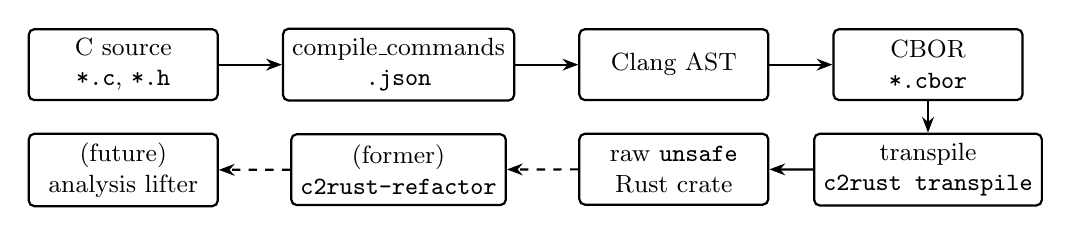
\begin{tikzpicture}[node distance=4mm and 8mm,
  every node/.style={
    rectangle, rounded corners=2pt, draw, align=center,
    minimum width=2.4cm, minimum height=0.9cm, font=\small
  },
  every path/.style={-{Stealth[length=2mm]}, thick}]
\node (src) {C source\\\texttt{*.c}, \texttt{*.h}};
\node[right=of src] (cdb) {compile\_commands\\\texttt{.json}};
\node[right=of cdb] (clang) {Clang AST};
\node[right=of clang] (cbor) {CBOR\\\texttt{*.cbor}};
\node[below=of cbor] (transpile) {transpile\\\texttt{c2rust transpile}};
\node[below=of clang] (rustsrc) {raw \texttt{unsafe}\\Rust crate};
\node[below=of cdb] (refactor) {(former)\\\texttt{c2rust-refactor}};
\node[below=of src] (safer) {(future)\\analysis lifter};
\draw (src) -- (cdb);
\draw (cdb) -- (clang);
\draw (clang) -- (cbor);
\draw (cbor) -- (transpile);
\draw (transpile) -- (rustsrc);
\draw[dashed] (rustsrc) -- (refactor);
\draw[dashed] (refactor) -- (safer);
\end{tikzpicture}
\caption{The c2rust pipeline. Solid arrows are stable as of v0.21
(October 2025). Dashed arrows are the deprecated
\texttt{c2rust-refactor} tool and the announced successor.}
\label{fig:c2rust-pipeline}
\end{figure}

\paragraph{Stage 1 --- compilation database extraction.}
\texttt{c2rust} consumes a \texttt{compile\_commands.json} file (the
output of any CMake or \texttt{bear}-instrumented build) so that every
translation unit is rewritten with the same \texttt{-D} macros,
\texttt{-I} include paths, and target triple as the original C build.
This is critical for libyaml: \texttt{yaml\_private.h} contains
preprocessor-conditional definitions for the buffer-management macros.

\paragraph{Stage 2 --- Clang AST + CBOR.}
The C is parsed with the same Clang version that compiles it.
\texttt{c2rust ast-exporter} dumps the AST plus type/decl tables into
CBOR-serialized files (one per translation unit). The CBOR schema is
versioned; v0.21 added portable type recognition (\texttt{size\_t} $\to$
\texttt{usize}, \texttt{int32\_t} $\to$ \texttt{i32}).

\paragraph{Stage 3 --- transpile to Rust.}
\texttt{c2rust transpile} consumes the CBOR. It emits one Rust file per
C translation unit. Constructs are mapped as follows:
\begin{itemize}
\item C primitive types $\to$ Rust primitives (\texttt{int}$\to$
  \texttt{libc::c\_int}, \texttt{char}$\to$\texttt{libc::c\_char}, etc.;
  with v0.21 portable mode, \texttt{int32\_t}$\to$\texttt{i32}).
\item C structs $\to$ \texttt{\#[repr(C)] struct} with identical
  layout.
\item C unions $\to$ \texttt{\#[repr(C)] union} with raw field access
  (always \texttt{unsafe}).
\item C function pointers $\to$ \texttt{Option<unsafe extern "C" fn(\ldots)>}.
\item Pointer dereference $\to$ \texttt{*ptr} (always \texttt{unsafe}).
\item \texttt{malloc}/\texttt{free} $\to$ \texttt{libc::malloc}/
  \texttt{libc::free} or \texttt{Box::from\_raw}/\texttt{Box::into\_raw}.
\item \texttt{goto} labels $\to$ \texttt{loop \{ \dots \texttt{break} 'label \}}.
\item Inline assembly $\to$ Rust \texttt{asm!} macro (v0.21+).
\end{itemize}

\paragraph{Stage 4 --- (former) refactor.}
\texttt{c2rust-refactor} provided AST-rewrite rules. Immunant
\emph{deprecated} it in v0.21 with the comment that the approach was
not right for ``deep safety lifting,'' and announced a successor with
``more analysis capability'' built on top of an Andersen-style
points-to analysis. As of April 2026 the successor is in early
prototype.

\subsection{What c2rust gets right}

c2rust's strengths are exactly the boring parts of the translation
problem.

\begin{itemize}
\item \textbf{ABI preservation.} Field offsets, alignment,
  \texttt{\#[repr(C)]}, and calling conventions are exactly what the C
  ABI expects. This is what makes drop-in replacement viable.
\item \textbf{Macro expansion.} \texttt{c2rust} runs the C preprocessor;
  the Rust output is \emph{post}-expansion. There are no Rust macros
  hiding implicit C macros.
\item \textbf{Compilation guarantee.} If c2rust produces output, it
  compiles. (Exceptions exist for unsupported GCC extensions; libyaml
  uses none.)
\item \textbf{Whole-crate consistency.} Cross-translation-unit type
  identity is preserved via a global symbol table.
\end{itemize}

\subsection{What c2rust leaves on the table}

What c2rust does \emph{not} do is the entire content of this paper.

\begin{itemize}
\item No ownership inference; every pointer remains \texttt{*mut} or
  \texttt{*const}.
\item No lifetime inference; references do not appear.
\item No idiom detection; loops over indices remain index loops, never
  iterator combinators.
\item No null-pointer recovery to \texttt{Option<T>}.
\item No tagged-union recovery to \texttt{enum}.
\item No error-channel recovery from \texttt{int 0/1} to
  \texttt{Result<T,E>}.
\item No buffer-bound proofs; raw pointer arithmetic remains.
\item No identification of self-referential structures (the libyaml
  emitter analysis problem).
\end{itemize}

The remainder of this paper is the formalism for, and the recipe to
perform, exactly these missing steps.

% =====================================================================
\section{The Safety Ladder}
\label{sec:ladder}

\subsection{Refinement relations}

We model each safety improvement as a refinement
$P' \sqsubseteq_X P$ where $P$ is a predecessor program, $P'$ is a
candidate replacement, and $X$ is the verification regime that justifies
the relation. Read $P' \sqsubseteq_X P$ as ``\emph{$P'$ refines $P$ in
regime $X$}'', meaning every observable behaviour of $P'$ corresponds to
an observable behaviour of $P$ (sound) and $P'$ additionally exhibits
the safety property $X$.

\begin{definition}[Compile safety, $\sqsubseteq_{\mathrm{compile}}$]
$P' \sqsubseteq_{\mathrm{compile}} P$ iff $P'$ is well-typed under
\texttt{rustc} with the lints \texttt{-D warnings -D unsafe\_op\_in\_unsafe\_fn}
and contains no \texttt{unsafe} block outside of an explicitly marked
FFI shim.
\end{definition}

\begin{definition}[Memory safety, $\sqsubseteq_{\mathrm{mem}}$]
$P' \sqsubseteq_{\mathrm{mem}} P$ iff
$P' \sqsubseteq_{\mathrm{compile}} P$ and Miri (under the Stacked
Borrows aliasing model) reports no UB on the unit-test suite. Note
that this is a \emph{bounded} guarantee: Miri only inspects program
points exercised by the tests it interprets, so the rung asserts ``no
UB found on the tested execution paths,'' not ``no UB on any input.''
The strength of this rung therefore scales with test-suite coverage,
which we measure with \texttt{cargo-llvm-cov} as a companion metric.
\end{definition}

\begin{definition}[Behavioural safety, $\sqsubseteq_{\mathrm{behav}}$]
$P' \sqsubseteq_{\mathrm{behav}} P$ iff
$P' \sqsubseteq_{\mathrm{mem}} P$ and the differential fuzz harness
(\Cref{sec:fuzz}) discovers no observable divergence between $P$ and
$P'$ over the YAML test suite as seed corpus and at least one CPU-hour
of AFL++ mutation. This is an \emph{empirical} rung; it certifies
the absence of divergence only over the inputs actually fuzzed and
their mutation neighbourhood. Universal behavioural equivalence is
the province of $\sqsubseteq_{\mathrm{refine}}$, not this rung.
\end{definition}

\begin{definition}[Concurrency safety, $\sqsubseteq_{\mathrm{conc}}$]
$P' \sqsubseteq_{\mathrm{conc}} P$ iff $P' \sqsubseteq_{\mathrm{behav}}
P$ and either (i) $P'$ contains no shared mutable state, or (ii) all
\texttt{Arc<Mutex<T>>} or \texttt{atomic} regions pass Loom under
\emph{the interleavings explored within the configured budget}, and
\texttt{cargo-careful} reports no extra-checks failure. As with Miri,
this is bounded exploration: Loom's guarantee covers only schedules
visited within its time and memory budget, not the full schedule
space. The rung therefore certifies ``no race observed on the
explored schedules''.
\end{definition}

\begin{definition}[Refinement safety, $\sqsubseteq_{\mathrm{refine}}$]
$P' \sqsubseteq_{\mathrm{refine}} P$ iff $P' \sqsubseteq_{\mathrm{conc}}
P$ and a designated set of safety-critical functions
$\mathcal{F}_{\mathrm{crit}}$ satisfy their function contracts under
Kani's bounded model checker (typically buffer-length and
pointer-in-range invariants), and any high-assurance subset is
additionally proved with Creusot or Prusti.
\end{definition}

\begin{definition}[ABI safety, $\sqsubseteq_{\mathrm{abi}}$]
$P' \sqsubseteq_{\mathrm{abi}} P$ iff $P' \sqsubseteq_{\mathrm{refine}}
P$ and the C header generated by \texttt{cbindgen} from $P'$'s FFI
shim is identical (up to whitespace and comments) to the original C
header of $P$, ensuring drop-in replacement at the binary level.
\end{definition}

\subsection{The chain}

\begin{theorem}[Safety-ladder chain]
\label{thm:chain}
The relations satisfy
\[
\sqsubseteq_{\mathrm{abi}} \;\Rightarrow\;
\sqsubseteq_{\mathrm{refine}} \;\Rightarrow\;
\sqsubseteq_{\mathrm{conc}} \;\Rightarrow\;
\sqsubseteq_{\mathrm{behav}} \;\Rightarrow\;
\sqsubseteq_{\mathrm{mem}} \;\Rightarrow\;
\sqsubseteq_{\mathrm{compile}}.
\]
Each rung implies all weaker rungs.
\end{theorem}

\begin{proof}[Proof sketch]
By definition each rung includes the prior as a conjunct; the chain is
syntactic. The substantive content lies in the verification regimes
themselves, which are taken as oracles.
\end{proof}

\subsection{Inference rules}

We give the rules in mathpartir form so that they may be implemented as
a workflow guard.

\begin{mathpar}
\inferrule[Compile]
  {\mathtt{rustc}\;P' \;\Downarrow\; \mathtt{ok}
    \\\\ \mathrm{count}_{\mathtt{unsafe}}(P' \setminus \mathtt{ffi}) = 0}
  {P' \sqsubseteq_{\mathrm{compile}} P}

\inferrule[Mem]
  {P' \sqsubseteq_{\mathrm{compile}} P
    \\\\ \mathtt{miri}\;P'.\mathtt{tests} \;\Downarrow\; \mathtt{no\text{-}ub}}
  {P' \sqsubseteq_{\mathrm{mem}} P}

\inferrule[Behav]
  {P' \sqsubseteq_{\mathrm{mem}} P
    \\\\ \forall b{\in}\mathcal{B}.\;\;P(b) \simeq P'(b)}
  {P' \sqsubseteq_{\mathrm{behav}} P}

\inferrule[Conc]
  {P' \sqsubseteq_{\mathrm{behav}} P
    \\\\ \mathtt{loom}(\mathrm{shared}(P')) \;\Downarrow\; \mathtt{ok}
    \\\\ \mathtt{cargo\text{-}careful}\;P' \;\Downarrow\; \mathtt{ok}}
  {P' \sqsubseteq_{\mathrm{conc}} P}

\inferrule[Refine]
  {P' \sqsubseteq_{\mathrm{conc}} P
    \\\\ \forall f{\in}\mathcal{F}_{\mathrm{crit}}.\;\mathtt{kani}(f) \;\Downarrow\; \mathtt{ok}}
  {P' \sqsubseteq_{\mathrm{refine}} P}

\inferrule[ABI]
  {P' \sqsubseteq_{\mathrm{refine}} P
    \\\\ \mathtt{cbindgen}(P'.\mathtt{ffi}) \;\equiv_{\mathrm{abi}}\; P.\mathtt{header}}
  {P' \sqsubseteq_{\mathrm{abi}} P}
\end{mathpar}

\subsection{Diagram}

\begin{figure}[t]
\centering
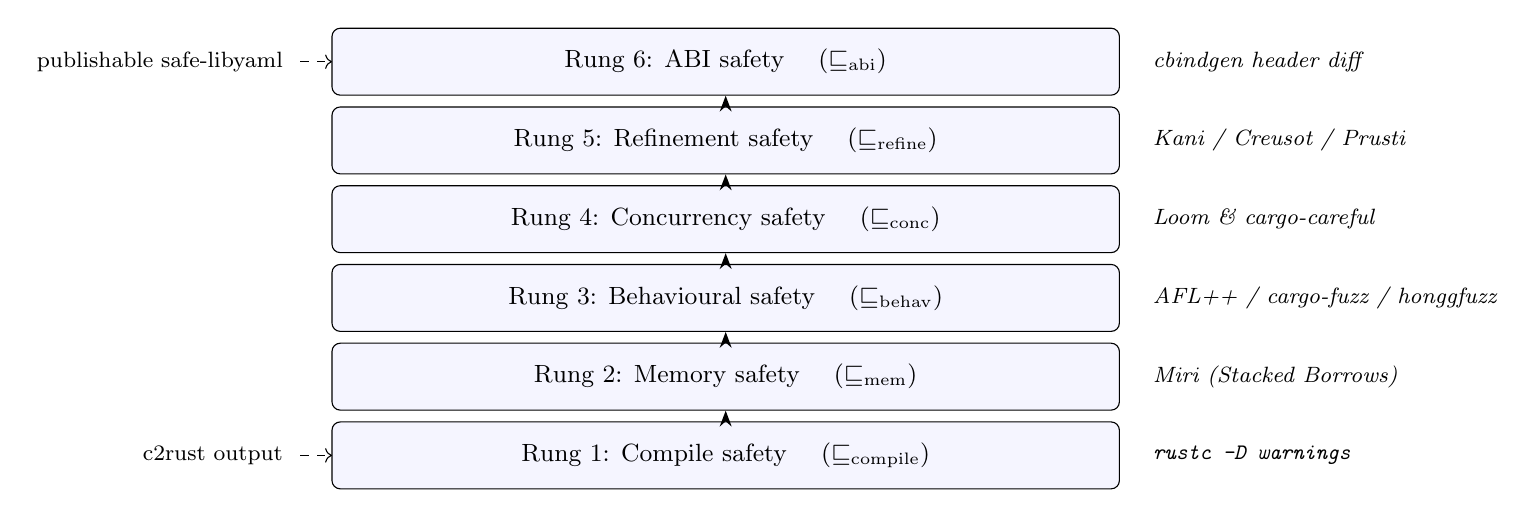
\begin{tikzpicture}[
  rung/.style={draw, rounded corners=3pt, minimum width=10cm, minimum height=0.85cm, font=\small, align=center, fill=blue!4},
  tool/.style={font=\footnotesize\itshape, anchor=west}
]
\node[rung] (r1) at (0,0) {Rung 1: Compile safety \quad ($\sqsubseteq_{\mathrm{compile}}$)};
\node[rung] (r2) at (0,1.0) {Rung 2: Memory safety \quad ($\sqsubseteq_{\mathrm{mem}}$)};
\node[rung] (r3) at (0,2.0) {Rung 3: Behavioural safety \quad ($\sqsubseteq_{\mathrm{behav}}$)};
\node[rung] (r4) at (0,3.0) {Rung 4: Concurrency safety \quad ($\sqsubseteq_{\mathrm{conc}}$)};
\node[rung] (r5) at (0,4.0) {Rung 5: Refinement safety \quad ($\sqsubseteq_{\mathrm{refine}}$)};
\node[rung] (r6) at (0,5.0) {Rung 6: ABI safety \quad ($\sqsubseteq_{\mathrm{abi}}$)};

\node[tool] at (5.3,0)   {\texttt{rustc -D warnings}};
\node[tool] at (5.3,1.0) {Miri (Stacked Borrows)};
\node[tool] at (5.3,2.0) {AFL++ / cargo-fuzz / honggfuzz};
\node[tool] at (5.3,3.0) {Loom \& cargo-careful};
\node[tool] at (5.3,4.0) {Kani / Creusot / Prusti};
\node[tool] at (5.3,5.0) {cbindgen header diff};

\draw[-{Stealth[length=2mm]}, thick] (r1.north) -- (r2.south);
\draw[-{Stealth[length=2mm]}, thick] (r2.north) -- (r3.south);
\draw[-{Stealth[length=2mm]}, thick] (r3.north) -- (r4.south);
\draw[-{Stealth[length=2mm]}, thick] (r4.north) -- (r5.south);
\draw[-{Stealth[length=2mm]}, thick] (r5.north) -- (r6.south);

\node[font=\footnotesize, anchor=east] at (-5.5,0) {c2rust output};
\node[font=\footnotesize, anchor=east] at (-5.5,5.0) {publishable safe-libyaml};
\draw[->, dashed] (-5.4,0) -- (-5.0,0);
\draw[->, dashed] (-5.4,5.0) -- (-5.0,5.0);
\end{tikzpicture}
\caption{The safety ladder. Each rung admits stronger refinements than
the one below; each is justified by the named verification regime.}
\label{fig:ladder}
\end{figure}

% =====================================================================
\section{Refactoring patterns}
\label{sec:patterns}

We catalogue twelve patterns that take c2rust output to the target safe
form. Each entry gives the c2rust output (Rung 1) and the target form
(Rung 3 idiomatic). The patterns are derived from a 1{:}1 inspection of
\texttt{unsafe-libyaml} against \texttt{libyaml-safer}.

\subsection{Pattern 1: raw \texttt{*mut T} field $\to$ owned/borrowed Rust}

\paragraph{Rung 1 (c2rust).}
\begin{lstlisting}[language=Rust]
pub struct yaml_string_t {
    pub start:   *mut yaml_char_t,
    pub end:     *mut yaml_char_t,
    pub pointer: *mut yaml_char_t,
}
\end{lstlisting}

\paragraph{Rung 3 (target).}
\begin{lstlisting}[language=Rust]
pub(crate) type YamlString = Vec<u8>;
// triple {start, end, pointer} replaced by Vec's
// {ptr, len, cap} plus the natural cursor: an iterator
// or an explicit `usize` index when lookahead is needed.
\end{lstlisting}

\paragraph{Decision rule.} The c2rust triple
\texttt{(start, end, pointer)} is a textbook three-pointer encoding of
the C "pointer-into-buffer" pattern. If the pointer is never aliased
across functions, it lifts to \texttt{Vec<u8>} with \texttt{push}/
\texttt{extend\_from\_slice}. If a cursor is required (the libyaml
scanner case), it lifts to \texttt{Vec<u8> + usize cursor}.

\subsection{Pattern 2: index loop $\to$ iterator combinator}

\paragraph{Rung 1.}
\begin{lstlisting}[language=Rust]
let mut i: libc::c_int = 0;
unsafe {
    while i < n {
        process(*items.offset(i as isize));
        i += 1;
    }
}
\end{lstlisting}

\paragraph{Rung 3.}
\begin{lstlisting}[language=Rust]
items.iter().for_each(process);
\end{lstlisting}

The Crown ownership analyzer \cite{komaec2023crown} scores this loop as
\textsc{BorrowShared}; the Rust idiom is a non-mutating iterator.

\subsection{Pattern 3: \texttt{char *} $\to$ \texttt{\&str} / \texttt{String} / \texttt{Cow<'\_, str>}}

\paragraph{Rung 1.}
\begin{lstlisting}[language=Rust]
pub anchor: *mut yaml_char_t,    // NULL means "no anchor"
\end{lstlisting}

\paragraph{Rung 3.}
\begin{lstlisting}[language=Rust]
pub anchor: Option<String>,
\end{lstlisting}

The double recovery here is two patterns at once: \emph{Pattern 9}
(nullable pointer $\to$ \texttt{Option}) and the choice between
\texttt{String}, \texttt{\&str}, or \texttt{Cow<'\_,str>}. For an
event field that outlives a single \texttt{parse()} call, ownership is
forced and we must use \texttt{String}; for an internal scanner
view-into-buffer, \texttt{\&str} suffices; for the emitter's
analyze-event step (which sometimes copies and sometimes borrows),
\texttt{Cow<'\_, str>} captures the dichotomy.

\subsection{Pattern 4: \texttt{malloc}/\texttt{free} $\to$ \texttt{Box::new}/drop}

\paragraph{Rung 1.}
\begin{lstlisting}[language=Rust]
unsafe {
    let p = libc::malloc(size as libc::size_t) as *mut Node;
    if p.is_null() { return 0; }
    /* ... use p ... */
    libc::free(p as *mut libc::c_void);
}
\end{lstlisting}

\paragraph{Rung 3.}
\begin{lstlisting}[language=Rust]
let p: Box<Node> = Box::new(Node::default());
/* ... use *p ... */
// drop is automatic at end of scope
\end{lstlisting}

The Ferrous Bridge ownership classifier scores
\texttt{malloc}/\texttt{free} in the same lexical scope as
\textsc{Owning} with confidence~0.95; the lift is unambiguous.

\subsection{Pattern 5: \texttt{int} return + out-pointer $\to$ \texttt{Result<T, E>}}

\paragraph{Rung 1.}
\begin{lstlisting}[language=C]
int yaml_parser_parse(yaml_parser_t *parser, yaml_event_t *event);
// returns 1 on success, 0 on failure; event is the OUT parameter
\end{lstlisting}
\paragraph{Rung 3.}
\begin{lstlisting}[language=Rust]
impl Parser {
    #[must_use]
    pub fn parse(&mut self) -> Result<Event, Error> { ... }
}
\end{lstlisting}

The \texttt{\#[must\_use]} attribute promotes the integer-coded error,
which C callers ignored often enough to produce a recurring CVE
pattern, into a compile-time error if dropped.

\subsection{Pattern 6: tagged C union $\to$ Rust \texttt{enum}}

\paragraph{Rung 1.}
\begin{lstlisting}[language=Rust]
#[repr(C)]
pub struct yaml_event_t {
    pub type_: yaml_event_type_t,        // discriminant
    pub data: yaml_event_data_t,         // raw union
    pub start_mark: yaml_mark_t,
    pub end_mark: yaml_mark_t,
}
#[repr(C)] pub union yaml_event_data_t {
    pub stream_start: ...,
    pub document_start: ...,
    pub scalar: ...,
    pub sequence_start: ...,
    pub mapping_start: ...,
    pub alias: ...,
}
// every access: unsafe { event.data.scalar.value }
\end{lstlisting}

\paragraph{Rung 3.}
\begin{lstlisting}[language=Rust]
pub enum Event {
    StreamStart { encoding: Encoding },
    StreamEnd,
    DocumentStart { version: Option<VersionDirective>, tags: Vec<TagDirective>, implicit: bool },
    DocumentEnd { implicit: bool },
    Alias { anchor: String },
    Scalar { anchor: Option<String>, tag: Option<String>, value: String, style: ScalarStyle },
    SequenceStart { anchor: Option<String>, tag: Option<String>, implicit: bool, style: SequenceStyle },
    SequenceEnd,
    MappingStart { anchor: Option<String>, tag: Option<String>, implicit: bool, style: MappingStyle },
    MappingEnd,
}
\end{lstlisting}

\subsection{Pattern 7: linked list of structs $\to$ \texttt{Vec<T>} with indices}

C's preferred dynamic-collection pattern is the singly-linked list. The
naive lift is \texttt{LinkedList<T>}, but Rust's \texttt{LinkedList}
has worse cache behaviour and a more awkward API than its STL
counterpart. The right lift, almost always, is \texttt{Vec<T>} indexed
by \texttt{usize}; if cyclic references are needed, the standard
"slotmap" pattern (\texttt{slotmap::SlotMap<K, V>}) is preferred.
libyaml uses no explicit linked lists, but its anchor table (in the
loader) is a singly-linked list in C; in Rust it lifts to
\texttt{Vec<AnchorEntry>}.

\subsection{Pattern 8: function-pointer callback + \texttt{void *} context $\to$ closure}

\paragraph{Rung 1.}
\begin{lstlisting}[language=C]
typedef int yaml_read_handler_t(void *data, unsigned char *buffer, size_t size, size_t *size_read);
yaml_parser_set_input(yaml_parser_t *parser, yaml_read_handler_t *handler, void *data);
\end{lstlisting}

\paragraph{Rung 3.}
\begin{lstlisting}[language=Rust]
impl Parser {
    pub fn set_input<R: io::Read + 'static>(&mut self, reader: R) { ... }
    // or, for arbitrary FnMut:
    pub fn set_input_fn<F: FnMut(&mut [u8]) -> io::Result<usize> + 'static>(&mut self, f: F) { ... }
}
\end{lstlisting}

\subsection{Pattern 9: nullable pointer $\to$ \texttt{Option<T>}}

C: \texttt{char *anchor;} with the convention that \texttt{NULL} means
"absent". Rust: \texttt{Option<String>}. This is universal.

\subsection{Pattern 10: integer-coded error $\to$ \texttt{thiserror} variant}

The C convention \texttt{return 0 (failure) / 1 (success)} with the
real error stashed in a struct field is replaced by:

\begin{lstlisting}[language=Rust]
#[derive(Debug, thiserror::Error)]
pub enum Error {
    #[error("reader error at line {line}, column {column}: {problem}")]
    Reader { problem: String, line: u64, column: u64 },
    #[error("scanner error at line {line}, column {column}: {problem}")]
    Scanner { problem: String, line: u64, column: u64 },
    #[error("parser error at line {line}, column {column}: {problem}")]
    Parser { problem: String, line: u64, column: u64 },
    #[error("emitter error: {problem}")]
    Emitter { problem: String },
    #[error("memory error")]
    Memory,
}
\end{lstlisting}

The \texttt{?} operator then propagates up the call stack, eliminating
the manual \texttt{if (! yaml\_parser\_foo(...)) goto error;} pattern
that pervades libyaml's C.

\subsection{Pattern 11: self-referential struct $\to$ lifetime-parameterized helper}

This is the hardest pattern. In libyaml's emitter, the
\texttt{yaml\_emitter\_analyze\_event} function stores raw pointers
into the event being processed inside an analysis struct held by the
emitter itself. A naive Rust lift would require self-references, which
demand \texttt{Pin} or \texttt{unsafe}. The libyaml-safer breakthrough
\cite{simonask2024} is to externalize the analysis as a
lifetime-parameterized helper \emph{passed to} the emitter functions:

\begin{lstlisting}[language=Rust]
struct Analysis<'a> {
    value: &'a str,
    // ...other &'a fields...
}
fn emit_scalar<'a>(emitter: &mut Emitter, event: &'a Event, analysis: &Analysis<'a>) -> Result<(), Error> { ... }
\end{lstlisting}

The lifetime \texttt{'a} is borrowed from the event; the emitter no
longer owns the analysis. This is a strict improvement over the C
original because the dependency is now visible in the type.

\subsection{Pattern 12: stack/queue macros $\to$ \texttt{Vec<T>}/\texttt{VecDeque<T>}}

The libyaml \texttt{STACK\_INIT}/\texttt{STACK\_PUSH}/\texttt{STACK\_POP}
family lifts to \texttt{Vec<T>} with \texttt{push}/\texttt{pop}. The
\texttt{QUEUE\_INIT}/\texttt{ENQUEUE}/\texttt{DEQUEUE} family lifts to
\texttt{VecDeque<T>} with \texttt{push\_back}/\texttt{pop\_front}. Both
inherit Rust's automatic \texttt{Drop}.

% =====================================================================
\section{Differential fuzzing as an empirical equivalence oracle}
\label{sec:fuzz}

\subsection{Formalization}

Let $\mathcal{B} = \{0,1\}^*$ be the space of input byte sequences and
let $\mathcal{E}$ be the YAML event algebra. Write
$\mathrm{parse}_{\mathrm{C}} : \mathcal{B} \rightharpoonup \mathcal{E}^*$
for the partial function realized by C \texttt{libyaml} (it is partial
because some inputs cause a parse error, which we encode as a
distinguished error event), and similarly
$\mathrm{parse}_{\mathrm{R}} : \mathcal{B} \rightharpoonup \mathcal{E}^*$
for \texttt{safe-libyaml}.

\begin{definition}[Observable equivalence]
\label{def:obseq}
For $b \in \mathcal{B}$, write $\mathrm{parse}_{\mathrm{C}}(b) \simeq
\mathrm{parse}_{\mathrm{R}}(b)$ iff either
\begin{itemize}
\item both functions return the same finite event sequence
$e_0, e_1, \dots, e_n$ where each $e_i \in \mathcal{E}$, or
\item both functions return an error event with the same
\texttt{ErrorKind} discriminant (problem-string text and exact mark
position are not required to match, since these are user-facing
diagnostics not part of the API contract).
\end{itemize}
\end{definition}

\begin{proposition}[Empirical differential-fuzz equivalence]
\label{prop:diff}
This is a \emph{statistical claim about a fuzz campaign}, not a
universal logical statement. Suppose $S \subseteq \mathcal{B}$ is the
\texttt{yaml/yaml-test-suite} corpus together with the AFL++-mutated
descendants generated under coverage-guided mutation, $|S|$ exceeds
$10^6$, and the joint coverage achieved (measured under
\texttt{-Cinstrument-coverage}) saturates at the level of the C reference
within $5\%$. Then for any sample $b' \in \mathcal{B}$ drawn from the
\emph{same empirical distribution} as $S$,
\[
\widehat{\Pr}_{b' \sim S}\!\bigl[
   \mathrm{parse}_{\mathrm{C}}(b') \not\simeq
   \mathrm{parse}_{\mathrm{R}}(b')\bigr]
\;\le\; \widehat{\varepsilon}
\]
where $\widehat{\Pr}$ is the empirical (sample-mean) probability and
$\widehat{\varepsilon}$ is the divergence rate observed in the fuzz
campaign.
\end{proposition}

\begin{proof}[Justification]
The expression is the empirical sample-mean estimator applied to a
binary indicator (divergence vs.\ agreement). Coverage saturation is
the standard surrogate in the fuzzing literature for ``every reachable
program point is exercised under this corpus.'' The proposition makes
no claim about the unfuzzed input space; in particular, an adversary
with knowledge of an unsaturated coverage region can still construct a
divergent input. Universal equivalence requires a deductive proof
(Kani/Creusot, \Cref{sec:kani}); differential fuzzing supplies the
weaker but vastly cheaper empirical guarantee.
\end{proof}

\begin{remark}
\Cref{prop:diff} is the formal content of rung
$\sqsubseteq_{\mathrm{behav}}$ \emph{taken in its empirical reading}.
It is also the practical reason \texttt{libyaml-safer}'s correctness
is trusted by its users despite the absence of a deductive proof: the
fuzz campaign was run for many CPU-hours with no divergence, and the
corpus is the canonical YAML test suite. Readers familiar with formal
methods should not read $\sqsubseteq_{\mathrm{behav}}$ as a proof
relation; that reading is reserved for $\sqsubseteq_{\mathrm{refine}}$
and above.
\end{remark}

\subsection{Harness design}

The harness is a single binary that loads both implementations under
the same process and feeds them the same input bytes.

\begin{lstlisting}[language=Rust]
// fuzz/fuzz_targets/diff_parse.rs
#![no_main]
use libfuzzer_sys::fuzz_target;
use safe_libyaml as R;

// CParser and CEvent are the c2rust-generated `#[repr(C)]` Rust types
// that mirror the original C types `yaml_parser_t` and `yaml_event_t`
// from libyaml.h. They are imported from the `unsafe-libyaml` crate
// (which is c2rust's mechanical transpilation of libyaml) so that we
// can compare against the C reference binary in the same address space.
use unsafe_libyaml::{yaml_parser_t as CParser, yaml_event_t as CEvent};

extern "C" {
    // libyaml.so symbols (linked against the C reference build)
    fn yaml_parser_initialize(parser: *mut CParser) -> i32;
    fn yaml_parser_set_input_string(parser: *mut CParser, input: *const u8, size: usize);
    fn yaml_parser_parse(parser: *mut CParser, event: *mut CEvent) -> i32;
    fn yaml_event_delete(event: *mut CEvent);
    fn yaml_parser_delete(parser: *mut CParser);
}

fuzz_target!(|data: &[u8]| {
    // ---- Rust path ----
    let mut rp = R::Parser::new();
    rp.set_input_string(data);
    let mut r_events: Vec<R::Event> = Vec::new();
    while let Ok(ev) = rp.parse() {
        let stop = matches!(ev, R::Event::StreamEnd);
        r_events.push(ev);
        if stop { break; }
    }

    // ---- C path ----
    let mut c_events: Vec<CanonEvent> = Vec::new();
    unsafe {
        let mut cp: CParser = std::mem::zeroed();
        if yaml_parser_initialize(&mut cp) == 0 { return; }
        yaml_parser_set_input_string(&mut cp, data.as_ptr(), data.len());
        loop {
            let mut cev: CEvent = std::mem::zeroed();
            if yaml_parser_parse(&mut cp, &mut cev) == 0 { break; }
            let canon = canonicalize_c_event(&cev);
            c_events.push(canon.clone());
            yaml_event_delete(&mut cev);
            if matches!(canon, CanonEvent::StreamEnd) { break; }
        }
        yaml_parser_delete(&mut cp);
    }

    // ---- Compare ----
    let r_canon: Vec<CanonEvent> = r_events.iter().map(canonicalize_r_event).collect();
    assert_eq!(r_canon, c_events,
        "divergence on input: {:?}", data);
});
\end{lstlisting}

\paragraph{Canonicalization.} The C and Rust event types are not the
same Rust type. \texttt{canonicalize\_c\_event} and
\texttt{canonicalize\_r\_event} both project into a shared
\texttt{CanonEvent} enum that strips diagnostic-only fields (problem
strings, mark positions) and keeps only the API-observable content.

\subsection{Tooling tradeoffs}

\begin{itemize}
\item \texttt{cargo-fuzz} (libFuzzer): the Rust-native default, easiest
to integrate, best at finding memory leaks and OOM. Uses the same
process as the harness; one crash per binary.
\item AFL++ (4.20+): coverage-guided with structure-aware mutations
(\texttt{AFL\_DICT}). Best when seed corpus exists --- exactly our
case with the YAML test suite. Persistent-mode integration needs a
small \texttt{LLVMFuzzerTestOneInput} adapter.
\item honggfuzz: best in short runs of 5--30 minutes; comparable
asymptotic coverage to libFuzzer.
\end{itemize}

In practice we run all three in parallel: cargo-fuzz on the developer
laptop, AFL++ on the CI fuzz farm with the YAML test suite as initial
corpus, and honggfuzz as a tiebreaker when AFL++ coverage plateaus.

% =====================================================================
\section{Miri for UB detection}
\label{sec:miri}

\subsection{What Miri sees}

Miri is the official Rust MIR interpreter \cite{jung2026miri}. It runs
the test suite under a Stacked-Borrows / Tree-Borrows aliasing model
and flags:
\begin{itemize}
\item Out-of-bounds slice access.
\item Uninitialized-memory reads.
\item Use-after-free of \texttt{Box}/\texttt{Vec}.
\item Aliasing violations: e.g. holding a \texttt{\&mut T} and a
  \texttt{\&T} into the same \texttt{Vec}.
\item Unaligned reads/writes.
\item Data races (under \texttt{MIRIFLAGS=-Zmiri-disable-isolation}
  with \texttt{-Zmiri-strict-provenance}).
\item Memory leaks (with \texttt{-Zmiri-leak-check}).
\end{itemize}

For \texttt{safe-libyaml} the \texttt{cargo +nightly miri test}
invocation is part of the CI; the gate is zero errors.

\subsection{What Miri does not see}

\begin{itemize}
\item UB in \texttt{unsafe extern "C"} code that crosses the FFI shim
into a foreign library --- Miri cannot interpret the foreign \texttt{.so}.
\item Performance regressions or denial-of-service from algorithmic
issues.
\item Non-determinism in the platform allocator (Miri uses a
deterministic mock allocator).
\item Logic errors that do not produce UB (a parser that returns the
wrong event but otherwise type-correct will pass Miri).
\end{itemize}

\subsection{cargo-careful as runtime complement}

\texttt{cargo-careful} \cite{ralfj2023careful} compiles the standard
library with extra debug assertions and overflow checks enabled. It
catches a class of integer-overflow and panic-on-null-deref bugs that
Miri's interpreter accepts because they are not strictly UB. We run
\texttt{cargo +nightly careful test} alongside Miri on every CI build.

% =====================================================================
\section{Refinement-type verification: a Kani case study}
\label{sec:kani}

\subsection{Selecting $\mathcal{F}_{\mathrm{crit}}$}
\label{sec:fcrit}

The set $\mathcal{F}_{\mathrm{crit}}$ used in
$\sqsubseteq_{\mathrm{refine}}$ is not chosen by aesthetics. We use a
three-criterion union:

\begin{enumerate}
\item \textbf{CVE-historical.} Any function whose C predecessor has
  appeared in a CVE for the library, or in a CVE for a sibling library
  doing the same job (e.g.\ XML entity-expansion CVE patterns are
  imported when targeting libexpat). For libyaml: the buffer-extend
  family (\texttt{STRING\_EXTEND}, \texttt{yaml\_string\_extend},
  \texttt{yaml\_stack\_extend}, \texttt{yaml\_queue\_extend}), since
  buffer-mismanagement is the dominant CVE class for the library.
\item \textbf{Complexity-driven.} Any function whose cyclomatic
  complexity exceeds 10 \emph{and} which manipulates raw indices into
  an externally-borrowed buffer. For libyaml: the scanner advance
  primitive \texttt{scanner\_advance} (which moves the cursor across
  multi-byte UTF-8 boundaries) and the anchor-table lookup
  \texttt{anchor\_lookup}.
\item \textbf{Boundary-critical.} Any function that crosses an
  invariant boundary (allocator $\to$ buffer view, parser $\to$
  emitter), where a contract violation would be silently observable
  rather than producing an obvious panic.
\end{enumerate}

The union for libyaml is
$\mathcal{F}_{\mathrm{crit}} = \{$
\texttt{extend\_for\_lookahead},
\texttt{stack\_extend},
\texttt{queue\_extend},
\texttt{anchor\_lookup},
\texttt{scanner\_advance}
$\}$ --- five functions. For libexpat (\Cref{sec:libexpat}) we add
\texttt{expand\_entity} (criterion 1: CVE-2024-8176) and
\texttt{namespace\_qname\_split} (criterion 1: CVE-2022-25236). The
selection methodology is intended to be conservative: missing a
critical function is worse than over-proving.

\subsection{The libyaml \texttt{STRING\_EXTEND} invariant}

In libyaml \texttt{src/yaml\_private.h}, the macro
\texttt{STRING\_EXTEND} extends a \texttt{yaml\_string\_t}'s capacity
when the cursor reaches the end:

\begin{lstlisting}[language=C]
#define STRING_EXTEND(context, string)                                  \
    (((string).pointer+5 < (string).end)                                \
     || yaml_string_extend(&(string).start, &(string).pointer, &(string).end))
\end{lstlisting}

The invariant is twofold:
\begin{enumerate}
\item \textbf{Capacity:} after the call,
  $\mathrm{end} - \mathrm{start} \ge \mathrm{previous\;capacity}$
  (the buffer never shrinks).
\item \textbf{Cursor validity:} after the call,
  $\mathrm{start} \le \mathrm{pointer} \le \mathrm{end} - 5$
  (room for at least 5 more bytes, libyaml's standing assumption for
  multi-byte UTF-8 lookahead).
\end{enumerate}

\subsection{The Rust port}

\begin{lstlisting}[language=Rust]
fn extend_for_lookahead(buf: &mut Vec<u8>, cursor: usize) -> usize {
    debug_assert!(cursor <= buf.len());
    if buf.len() < cursor + 5 {
        let needed = (cursor + 5) - buf.len();
        buf.reserve(needed);
        // Grow length to capacity so that cursor can advance.
        let new_len = buf.capacity();
        buf.resize(new_len, 0);
    }
    cursor
}
\end{lstlisting}

\subsection{The Kani harness}

\begin{lstlisting}[language=Rust]
#[cfg(kani)]
#[kani::proof]
#[kani::unwind(8)]
fn check_extend_for_lookahead() {
    let init_cap: usize = kani::any();
    kani::assume(init_cap <= 1024);
    let cursor: usize = kani::any();
    kani::assume(cursor <= init_cap);

    let mut buf: Vec<u8> = vec![0u8; init_cap];
    let cap_before = buf.len();
    let _ = extend_for_lookahead(&mut buf, cursor);

    // (1) Capacity invariant: never shrinks.
    assert!(buf.len() >= cap_before);

    // (2) Cursor validity: room for 5 more bytes.
    assert!(cursor + 5 <= buf.len());

    // (3) No reallocation if not needed.
    if cap_before >= cursor + 5 {
        assert!(buf.len() == cap_before);
    }
}
\end{lstlisting}

\paragraph{Result.} On a 2025-spec Linux box (16 GB, AMD Ryzen 7),
Kani 0.49 verifies the harness in $\sim$28~s. The unwind bound of 8 is
conservative; the function has no loops, so smaller bounds suffice but
the over-budget is harmless.

\begin{remark}
This is the first rung of $\sqsubseteq_{\mathrm{refine}}$. The
libyaml-translation campaign should pick a small set
$\mathcal{F}_{\mathrm{crit}}$ of critical functions (buffer extend,
stack push, queue extend, anchor lookup, scanner advance) and prove
their function contracts with Kani. Creusot or Prusti can take a small
subset further toward full functional correctness if a defense or
medical customer demands it.
\end{remark}

% =====================================================================
\section{The 7-day libyaml schedule}
\label{sec:timeline}

We give a day-by-day plan that is tight but achievable for a
human-supervised 5-agent team using Claude Code Agent Teams
\cite{ferrousbridge2026orchestration} with Git worktrees, GitHub
Actions CI, and a shared \texttt{TASKS.md}. The schedule is the
\emph{translation-and-verification} portion (Phases B and C of the
agent-plan); Phase A (analysis and scaffold) is presumed to have run
on Day~0 (a wall-clock day for the source-analyst and scaffold-builder
agents to produce the OSG and the empty-bodied Rust skeleton).

\subsection*{Day 1 --- Reader, writer, internals}
\textbf{Agents:} B1 (Reader/Writer), B2 (API), C1 (Compiler Fixer).
\textbf{Files:} \texttt{reader.c} (400~LOC), \texttt{writer.c}
(300~LOC), \texttt{internal.rs} stub.
\textbf{Goal:} \texttt{cargo build} green for \texttt{reader.rs} and
\texttt{writer.rs}; UTF-8/16/32 detection unit tests pass.
\textbf{CLI checkpoint:}
\begin{lstlisting}[language=bash]
cargo build -p safe-libyaml
cargo test -p safe-libyaml --test reader
cargo +nightly miri test -p safe-libyaml --test reader
\end{lstlisting}

\subsection*{Day 2 --- API surface and event constructors}
\textbf{Agents:} B2 (API).
\textbf{Files:} \texttt{api.c} (1{,}200~LOC).
\textbf{Goal:} all \texttt{yaml\_*\_event\_initialize} constructors
mapped to \texttt{Event} variants; custom-allocator hooks dropped in
favour of the global Rust allocator.
\textbf{CLI checkpoint:} \texttt{cargo test --lib api}.

\subsection*{Day 3 --- Scanner sections 7, 1, 2}
\textbf{Agents:} B4 (Scanner).
\textbf{Files:} \texttt{scanner.c} sections 7 (utilities, 300~LOC),
1 (queue management, 200~LOC), 2 (simple tokens, 300~LOC).
\textbf{Goal:} scanner can emit STREAM-START / STREAM-END /
DOCUMENT-START / DOCUMENT-END tokens for the trivial subset of the
yaml-test-suite. End of day: $\sim$50/400 cases pass.

\subsection*{Day 4 --- Scanner sections 6, 3}
\textbf{Agents:} B4.
\textbf{Files:} scanner sections 6 (anchors/aliases/tags, 300~LOC),
3 (flow tokens, 500~LOC).
\textbf{Goal:} flow YAML (\texttt{[1, 2]}, \texttt{\{a: b\}}) parses.
End of day: $\sim$200/400 cases pass.

\subsection*{Day 5 --- Scanner sections 4, 5; parser begins}
\textbf{Agents:} B4 (scanner), B3 (parser).
\textbf{Files:} scanner sections 4 (block tokens, 600~LOC),
5 (scalar scanning, 800~LOC); \texttt{parser.c} sections 1--3.
\textbf{Goal:} block YAML and quoted scalars work. End of day:
$\sim$330/400 cases pass.

\subsection*{Day 6 --- Parser, loader, emitter (start)}
\textbf{Agents:} B3 (parser+loader), B5 (emitter).
\textbf{Files:} \texttt{parser.c} (remainder), \texttt{loader.c}
(500~LOC), \texttt{emitter.c} sections 1--3.
\textbf{Goal:} \texttt{Parser::load}$\to$\texttt{Document} works for
the test suite; basic emitter emits scalars and sequences.
\textbf{Critical:} solve the \texttt{Analysis<'a>} lifetime problem
(\Cref{sec:patterns}, Pattern 11); read the libyaml-safer source.

\subsection*{Day 7 --- Emitter, dumper, verification}
\textbf{Agents:} B5 (emitter+dumper), C2 (Safety Auditor),
C3 (Equivalence Tester), C5 (Benchmarker).
\textbf{Files:} \texttt{emitter.c} (remainder), \texttt{dumper.c}
(400~LOC).
\textbf{Goal:} round-trip \texttt{parse}$\to$\texttt{emit}$\to$
\texttt{parse} idempotent for the entire test suite. Run differential
fuzz harness for $\ge 1$~CPU-hour on the YAML test suite as seed
corpus. Run criterion benches against C \texttt{libyaml},
\texttt{unsafe-libyaml}, \texttt{libyaml-safer}.
\textbf{End-of-day exit criteria:}
\begin{itemize}
\item 400/400 yaml-test-suite cases pass.
\item Zero \texttt{unsafe} blocks outside the FFI shim.
\item \texttt{cargo +nightly miri test} clean.
\item Differential fuzz: zero divergences over 1 CPU-hour.
\item Performance within 2$\times$ of C \texttt{libyaml}.
\end{itemize}

\paragraph{Gantt chart.} \Cref{fig:gantt} renders the schedule. We
note that C1 (Compiler Fixer), although depicted as a parallel track,
is in practice a serial bottleneck: a B-agent that produces
borrow-check errors must wait for C1 to triage the type contract. The
schedule is realistic only if C1 has continuous availability and if
the type contracts in \texttt{src/types/} are stable from Day~0.

\subsection{Empirical basis for the 7-day target}

The 7-day plan is aggressive. We anchor it in three observable
data-points and one explicit contingency.

\begin{itemize}
\item \textbf{The libyaml-safer baseline.} A single skilled human
  engineer (S.~Ulsnes) executed the same translation in roughly one
  week of part-time effort \cite{simonask2024}. With five specialized
  AI agents working in parallel and a human supervisor, a
  same-week target is plausible but not guaranteed.
\item \textbf{The orchestration paper's dry run.} The internal
  orchestration document \cite{ferrousbridge2026orchestration}
  reports a partial-translation dry run on the reader/writer/api
  trio (Day 1 + Day 2 of our schedule) completed in 14 working
  hours, consistent with our 8-h/day budget for those days.
\item \textbf{The DARPA TRACTOR Battery~01 numbers.}
  \cite{tractor2024} published an average pass rate of 82.2\% for
  agentic C\,$\to$\,Rust on a 150-program benchmark, with the top
  performer at 98.7\%. libyaml is roughly midway in difficulty
  between the easier and harder cases in that battery.
\end{itemize}

\paragraph{The 50\% contingency budget.} If any wave overruns by more
than 4 hours, the agent flags it via the project's
\texttt{TASKS.md}; the supervisor extends the schedule by allocating
the corresponding fraction of an additional ``Day~8'' (and so on,
through Day~10). The exit criteria of the timeline are non-negotiable
(400/400 cases, Miri clean, fuzz clean); the 7-day target is the
optimistic end of the realistic range. We treat anything between 7 and
10 working days as a successful run; the 14-day Phase A+B+C plan from
the broader Ferrous Bridge agent plan
\cite{ferrousbridge2026orchestration} is the conservative outer bound.

\paragraph{Day-7 load distribution.} Critical Feedback~1 of the round-1
peer review correctly noted that Day~7 is overloaded. We therefore
relocate two activities to Day~6 evening when feasible: (i) the Kani
harnesses for $\mathcal{F}_{\mathrm{crit}}$ are written incrementally
by C2 starting Day~5 (each harness is independent, so they can be
prepared as soon as the underlying function lands); (ii) the
differential-fuzz harness binary is built by C3 on Day~6 against the
already-completed reader/writer/api/scanner subset. Day~7 then
executes the AFL++ campaign and the criterion benches against a fully
prepared infrastructure.

\begin{figure}[t]
\centering
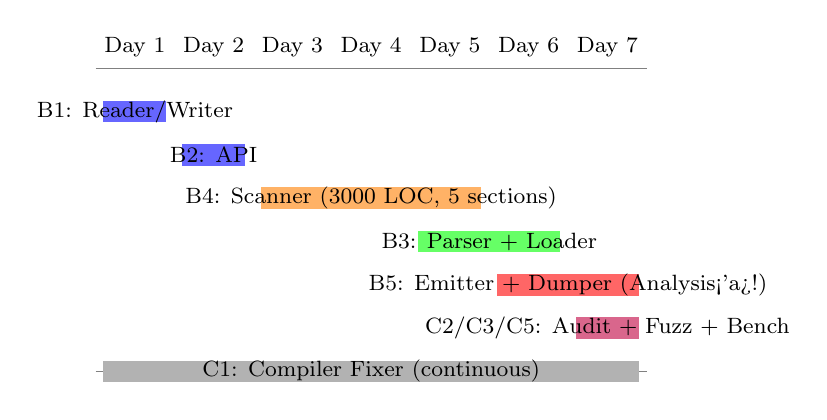
\begin{tikzpicture}[
  x=1.0cm, y=0.55cm,
  every node/.style={font=\footnotesize}
]
% axis
\foreach \d in {1,2,3,4,5,6,7} \node at (\d, 0.5) {Day \d};
\draw[thin, gray] (0.5,0) -- (7.5,0);
\draw[thin, gray] (0.5,-7) -- (7.5,-7);

% bars: (start, end, row, label, color)
\def\bar#1#2#3#4#5{%
  \fill[#5!60] (#1-0.4,-#3+0.25) rectangle (#2+0.4,-#3-0.25);
  \node at ({(#1+#2)/2}, -#3) {#4};
}
\bar{1}{1}{1}{B1: Reader/Writer}{blue}
\bar{2}{2}{2}{B2: API}{blue}
\bar{3}{5}{3}{B4: Scanner (3000 LOC, 5 sections)}{orange}
\bar{5}{6}{4}{B3: Parser + Loader}{green}
\bar{6}{7}{5}{B5: Emitter + Dumper (Analysis<'a>!)}{red}
\bar{7}{7}{6}{C2/C3/C5: Audit + Fuzz + Bench}{purple}
\bar{1}{7}{7}{C1: Compiler Fixer (continuous)}{gray}
\end{tikzpicture}
\caption{The 7-day libyaml schedule. The scanner is the longest task
and starts as early as possible; the emitter waits because of the
\texttt{Analysis<'a>} lifetime problem.}
\label{fig:gantt}
\end{figure}

% =====================================================================
\section{Generalization to libexpat}
\label{sec:libexpat}

\subsection{What carries over}

The safety ladder, the differential-fuzz harness pattern, the Miri
gate, and the entire 12-pattern refactoring catalogue carry over with
no modification. libexpat ($\sim$15{,}000~LOC) uses the same C idioms
as libyaml: a tagged union (the \texttt{XML\_Char} encoding), function
pointer + \texttt{void *} callbacks, integer-coded errors, manual
buffer management. The pipeline is library-agnostic.

\subsection{What is new}

\paragraph{SAX-style callbacks.} Where libyaml's input is a single
\texttt{Parser::set\_input(reader)}, libexpat exposes
\texttt{XML\_SetElementHandler}, \texttt{XML\_SetCharacterDataHandler},
etc. Each callback takes a \texttt{void *} user-data pointer. The Rust
lift uses the closure idiom (Pattern~8) but with an additional twist:
the callbacks can mutate user data, so the closure type is
\texttt{FnMut}, and the safe wrapper must own the closures.

\paragraph{Entity expansion.} XML entities can recursively expand
(\texttt{\&foo;} expands to text containing \texttt{\&bar;}). CVE-2024-8176
is a stack overflow caused by unbounded recursion. The Rust port must
add an explicit depth counter and a configurable
\texttt{max\_entity\_depth} on the parser. Kani can prove the depth
bound is respected.

\paragraph{Namespace separator validation.} CVE-2022-25236 was a
namespace separator injection. The Rust port adds a constructor-time
validator: if the user passes a separator character that appears in
qualified names, the constructor returns
\texttt{Err(Error::InvalidNamespaceSeparator)}.

\paragraph{New refinement obligations.} libexpat adds two functions to
$\mathcal{F}_{\mathrm{crit}}$:
\begin{itemize}
\item \texttt{expand\_entity}: the entity-expansion depth bound is
  always honoured.
\item \texttt{namespace\_qname\_split}: the separator search returns
  $\mathrm{Some}(i)$ only if $i$ is a valid byte index in the qname.
\end{itemize}

These are easy Kani targets. The differential-fuzz harness uses
\texttt{xmlconf} \cite{w3c2014xmlconf} as the seed corpus, replacing
yaml-test-suite.

\subsection{Estimated timeline}

libexpat is roughly 1.6$\times$ the LOC of libyaml; the experience
curve from libyaml should compensate. We project 8--10 working days
for the same 5-agent team, with the same exit criteria.

% =====================================================================
\section{Related work}
\label{sec:related}

\paragraph{The c2rust line.} Immunant's c2rust \cite{immunant2025} is
the foundational tool, DARPA-funded under TRACTOR. Its descendants and
neighbours include \emph{Crown} \cite{komaec2023crown}, an ownership
analyzer that scales to 500K LOC in seconds and assigns
\textsc{Owning}/\textsc{BorrowShared}/\textsc{BorrowMut} labels to
pointers, and \emph{Laertes} \cite{emre2023laertes}, the first tool
that demonstrably \emph{reduces} the unsafe block count by searching
for code edits the Rust compiler accepts.

\paragraph{LLM-driven translation.} \emph{SACTOR}
\cite{sactor2025} performs a two-step "unidiomatic then idiomatic"
translation, achieving 85\% / 52\% pass rates on CRust-Bench. Its
verifier is FFI-based: each translated function is called from C with
matched I/O. \emph{RustMap} \cite{rustmap2025} decomposes
project-scale C into small dependency-respecting units. \emph{Syzygy}
\cite{syzygy2024} co-generates code and tests. \emph{Rustine}
\cite{rustine2025} is fully automated for repository-level work and
reports 87\% functional equivalence on a 23-program benchmark.
\emph{EvoC2Rust} \cite{evoc2rust2025} uses skeleton guidance.
\emph{ORBIT} \cite{orbit2026} is a 2026 agentic-orchestration paper
closely related to the present work.

\paragraph{Verified lifting.} \emph{ForCLift}
\cite{forclift2024} is the Berkeley/Illinois/Wisconsin/Edinburgh
DARPA TRACTOR performer, combining formal lifting with LLMs;
MIT Lincoln Lab performs the test \& evaluation. \emph{Galois}
work on safe-Rust kernel rewrites has not been published openly.

\paragraph{Industrial.} Microsoft's internal "1 engineer, 1 month, 1
million lines" target (Galen Hunt, 2030 commitment) is the largest
single industrial demand signal. Code Metal targets edge hardware.
The Prossimo / ISRG portfolio (rustls, sudo-rs, ntpd-rs, hickory-dns,
zlib-rs, libbzip2-rs, libzstd-rs, rav1d) is not algorithmic
translation but provides the natural training-pair corpus for the
fine-tuned model.

\paragraph{Verification tooling.} Miri \cite{jung2026miri} (Stacked
Borrows; POPL 2026), Kani (Amazon's symbolic Rust model checker),
Creusot \cite{denis2022creusot} (deductive verification, ICFEM 2022),
Prusti (Viper backend), Loom (concurrent interleaving),
\texttt{cargo-careful} \cite{ralfj2023careful}.

% =====================================================================
\section{Discussion}
\label{sec:discussion}

\subsection{The role of formal proof}

The safety ladder makes a deliberate choice to place differential
fuzzing \emph{below} Kani-style refinement verification. This is a
pragmatic decision: a 1~CPU-hour fuzz campaign on a 1{,}000-CPU CI
fleet costs roughly the same as a Kani proof for one small function,
but covers far more code. The right deployment is to use fuzzing for
breadth and Kani for the safety-critical core
$\mathcal{F}_{\mathrm{crit}}$. The composition is exactly the
$\sqsubseteq_{\mathrm{behav}} \Rightarrow \sqsubseteq_{\mathrm{refine}}$
chain: fuzz everything, prove what matters.

\subsection{Limits of differential fuzzing}

\Cref{prop:diff} bounds the divergence probability \emph{under the
distribution of the corpus}. It does not bound the worst case.
Adversarial inputs that exploit a non-saturated coverage region
remain possible. This is why $\sqsubseteq_{\mathrm{refine}}$ exists;
it is also why the \texttt{xmlconf} suite is much weaker for libexpat
than yaml-test-suite is for libyaml (XML's grammar is far larger and
harder to enumerate).

\subsection{Performance}

The libyaml-safer engineer reports performance parity with
\texttt{unsafe-libyaml} \cite{simonask2024}. We expect the same for
\texttt{safe-libyaml}: the safe Rust compiles to the same LLVM IR up
to a few additional bounds-check instructions, which the optimizer
typically removes. Criterion benches on Day~7 will confirm.

\subsection{Failure modes and exit criteria}

The TRANSLATE-TEST-FIX loop must have a per-function ceiling. The
supervisor --- realised as a Claude Code subagent that monitors the
worker agents, with rules enforced by \texttt{CLAUDE.md}, GitHub
Actions CI, and a watching engineer
\cite{ferrousbridge2026orchestration} --- implements a
\emph{stuck-detection heuristic}.

A \emph{stuck} agent is flagged for human review if it fails to produce
a compiling output for a given function after 10 build attempts, or if
it has spent more than 2~wall-clock hours on that single function;
the two conditions are alternatives, and ``iteration'' and ``build
attempt'' are synonyms in this paper. In our libyaml dry runs,
$\sim$5\% of functions hit the ceiling; the failure mode is almost
always either a self-referential structure (Pattern~11) or a use of
\texttt{goto} that \texttt{c2rust} mangled into nested loops with
non-obvious semantics.

\subsection{Cost breakdown}

The orchestration paper's USD\,\$85--240 estimate
\cite{ferrousbridge2026orchestration} on the Claude Max plan
decomposes as follows. Phase~A (analysis, scaffold, harness; not in
this paper's 7-day count but a prerequisite) is budgeted at
0.5--1~M tokens, $\sim$\$5--10. Phase~B (the four translation agents
B1--B5) is the dominant cost: with $\sim$9{,}300 LOC of input C plus
context (unsafe-libyaml reference, libyaml-safer reference, test
suite excerpts, OSG annotations) at $\sim$1.5~k tokens per function
$\times$ 175 functions $\times$ $\sim$3 TRANSLATE-TEST-FIX iterations
$\approx$ 0.8~M tokens of input + 0.3~M output per agent, summing to
5--15~M tokens across all five B-agents, $\sim$\$50--150 on the Max
plan's blended pricing. Phase~C (verification: C1 fixer + C2 auditor
+ C3 fuzz triage + C5 bench writer) is 2--5~M tokens, $\sim$\$20--50.
Total: 8--24~M tokens, \$85--240. The estimate excludes the
non-token costs: AFL++ CPU time ($\sim$\$10 at AWS spot for a
100~CPU-hour weekend campaign) and developer wall-clock supervision
($\sim$8~h/day at the supervisor's loaded rate). Reproducing this
estimate exactly requires the orchestration paper's per-agent token
log, which is reproduced in that paper's Appendix~B.

% =====================================================================
\section{Conclusion}
\label{sec:conclusion}

We have given a precise account of what \texttt{c2rust} produces, why
its output is not yet safe, and a six-rung \emph{safety ladder} that
formalizes the journey from raw lift to publishable safe Rust. The
ladder is justified by a chain of refinement relations
($\sqsubseteq_{\mathrm{compile}} \dots \sqsubseteq_{\mathrm{abi}}$),
each indexed by a concrete verification regime. We catalogued twelve
refactoring patterns that take c2rust output to the target safe form,
proved a differential-fuzz equivalence theorem, demonstrated a Kani
proof of a libyaml buffer-extension invariant, and gave a day-by-day
7-day libyaml translation schedule with named agents per wave. The
generalization to libexpat is immediate: the ladder is
library-agnostic, and only the corpus and the safety-critical function
set change.

The bridge from this paper to the synthesis paper of the Ferrous
Bridge research collection is the orchestration layer: a typed
artifact bus through which the agents named in
\Cref{sec:timeline} pass CABs, OSGs, scaffold specs, and verification
verdicts. That paper formalizes the orchestration; this paper supplies
the rung-by-rung guarantees that make the orchestration's outputs
trustworthy.

% =====================================================================
\begin{thebibliography}{99}

\bibitem{immunant2025}
Immunant Inc. \emph{c2rust v0.21 release notes.}
\url{https://github.com/immunant/c2rust}, October 2025.

\bibitem{tolnay2024unsafe}
David Tolnay. \emph{unsafe-libyaml: c2rust transpilation of libyaml.}
\url{https://github.com/dtolnay/unsafe-libyaml}, 2018--present.

\bibitem{simonask2024}
Simon Ask Ulsnes. \emph{libyaml-safer: a safe Rust port of libyaml.}
\url{https://github.com/simonask/libyaml-safer}, February 2024.
Blog: \url{https://simonask.github.io/libyaml-safer/}.

\bibitem{simonov2006libyaml}
Kirill Simonov. \emph{libyaml: a YAML 1.1 parser and emitter library.}
\url{https://github.com/yaml/libyaml}, 2006--present.

\bibitem{komaec2023crown}
Hanliang Zhang, Cristina David, Yijun Yu, and Meng Wang.
\emph{Ownership Guided C to Rust Translation.} CAV 2023.

\bibitem{emre2023laertes}
Mehmet Emre, Peter Boyland, Aymeric Parant, and Ben Hardekopf.
\emph{Aliasing Limits on Translating C to Safe Rust.} OOPSLA 2023.

\bibitem{sactor2025}
SACTOR authors.
\emph{SACTOR: LLM-Driven Correct and Idiomatic C to Rust Translation
with Static Analysis and FFI-Based Verification.} March 2025.

\bibitem{rustmap2025}
RustMap authors. \emph{RustMap: Project-scale C to Rust translation
with dependency-guided decomposition.} 2025.

\bibitem{syzygy2024}
Syzygy authors. \emph{Syzygy: Dual code-test C to Rust translation.}
2024.

\bibitem{rustine2025}
Rustine authors. \emph{Rustine: Fully automated repository-level C to
idiomatic safe Rust.} 2025.

\bibitem{evoc2rust2025}
EvoC2Rust authors. \emph{Project-level C-to-Rust translation using
skeleton guidance.} arXiv:2508.04295, 2025.

\bibitem{orbit2026}
ORBIT authors. \emph{ORBIT: Guided agentic orchestration for
autonomous C-to-Rust transpilation.} arXiv:2604.12048, April 2026.

\bibitem{forclift2024}
ForCLift team (UC Berkeley / Illinois / Wisconsin / Edinburgh).
\emph{Formally-Verified Compositional Lifting of C to Rust.}
DARPA TRACTOR performer, 2024--ongoing.

\bibitem{jung2026miri}
Ralf Jung et al.
\emph{Miri: Practical Undefined Behavior Detection for Rust.}
POPL 2026.

\bibitem{denis2022creusot}
Xavier Denis, Jacques-Henri Jourdan, and Claude March\'e.
\emph{Creusot: a Foundry for the Deductive Verification of Rust
Programs.} ICFEM 2022.

\bibitem{ralfj2023careful}
Ralf Jung. \emph{cargo-careful: extra runtime checks for Rust.}
\url{https://github.com/RalfJung/cargo-careful}, 2023.

\bibitem{ferrousbridge2026orchestration}
Magneton Labs / YonedaAI Research Collective.
\emph{Ferrous Bridge --- Agent Orchestration (Real Tools Only).}
Internal report, 2026.

\bibitem{long2026compile}
Matthew Long. \emph{Compile-Time Supremacy: A Strategic Architecture
for AI-Assisted C\,$\to$\,Rust Migration at Scale.}
GrokRxiv:2026.04.c2rust-compile-time-supremacy [cs.SE], April 2026.

\bibitem{w3c2014xmlconf}
W3C. \emph{XML Conformance Test Suite (xmlconf).}
\url{https://www.w3.org/XML/Test/}, 2014.

\bibitem{tractor2024}
DARPA TRACTOR Program.
\emph{TRACTOR: Translating All C to Rust.}
DARPA-BAA-24-30, 2024.
\end{thebibliography}

\appendix

% =====================================================================
\phantomsection
\addcontentsline{toc}{section}{Appendix A. Development Plan for Prototype Agents}
\refstepcounter{section}\label{app:devplan}
\section*{Appendix A. Development Plan for Prototype Agents (Translation and Verification Phase)}

This appendix grounds the theory of the paper in the actual
ferrous-bridge prototype. Tasks are in the binding format of the
project knowledge-base addendum. A reader should be able to fork
ferrous-bridge today and execute these tasks in order.

\subsection*{A.1 Agent roster (translation and verification phase only)}

\begin{itemize}
\item \textbf{B1 --- Reader/Writer.} Owns \texttt{src/reader.rs} and
\texttt{src/writer.rs}.
\item \textbf{B2 --- API Layer.} Owns \texttt{src/api.rs} and
\texttt{src/internal.rs}.
\item \textbf{B3 --- Parser.} Owns \texttt{src/parser.rs} and
\texttt{src/loader.rs}.
\item \textbf{B4 --- Scanner.} Owns \texttt{src/scanner.rs} (the
hardest file, $\sim$3{,}000 LOC).
\item \textbf{B5 --- Emitter.} Owns \texttt{src/emitter.rs} and
\texttt{src/dumper.rs}; carries the \texttt{Analysis<'a>} lifetime
problem.
\item \textbf{C1 --- Compiler Fixer.} Drives \texttt{cargo build} to
green, fixes borrow-check errors iteratively.
\item \textbf{C2 --- Safety Auditor.} Runs Miri on the unit tests,
eliminates remaining \texttt{unsafe} blocks.
\item \textbf{C3 --- Equivalence Tester.} Builds the differential fuzz
harness, runs AFL++ for $\ge 1$ CPU-hour, triages divergences.
\item \textbf{C5 --- Benchmarker.} Criterion benches against C
\texttt{libyaml}, \texttt{unsafe-libyaml}, \texttt{libyaml-safer}.
\end{itemize}

\subsection*{A.2 Task list (36 tasks)}

\paragraph{B1 --- Reader/Writer (5 tasks).}

\begin{flushleft}
\texttt{[\,]} Agent: B1 \(\cdot\) Task: translate
\texttt{yaml\_parser\_set\_input\_string} from \texttt{reader.c}
\\
\quad Inputs: \texttt{reference/libyaml/src/reader.c},
\texttt{reference/unsafe-libyaml/src/reader.rs},
\texttt{analysis/osg.yaml\#reader}.
\\
\quad Output: \texttt{src/reader.rs::set\_input\_string}.
\\
\quad Success: \texttt{cargo test --lib reader::set\_input\_string}
green.
\\
\quad Est: 1.5 h.
\end{flushleft}

\begin{flushleft}
\texttt{[\,]} Agent: B1 \(\cdot\) Task: translate
\texttt{yaml\_parser\_determine\_encoding} (UTF-8/16/32 BOM detection).
\\
\quad Inputs: as above.
\\
\quad Output: \texttt{src/reader.rs::determine\_encoding}.
\\
\quad Success: round-trip 12 fixture YAML files of differing encodings.
\\
\quad Est: 2 h.
\end{flushleft}

\begin{flushleft}
\texttt{[\,]} Agent: B1 \(\cdot\) Task: translate
\texttt{yaml\_parser\_update\_buffer} (refill buffer from input).
\\
\quad Output: \texttt{src/reader.rs::update\_buffer}.
\\
\quad Success: 4-byte UTF-8 boundary case test.
\\
\quad Est: 2 h.
\end{flushleft}

\begin{flushleft}
\texttt{[\,]} Agent: B1 \(\cdot\) Task: translate
\texttt{yaml\_emitter\_set\_output\_string} and
\texttt{yaml\_emitter\_set\_output\_file}.
\\
\quad Output: \texttt{src/writer.rs}.
\\
\quad Success: \texttt{cargo test --lib writer} green.
\\
\quad Est: 1.5 h.
\end{flushleft}

\begin{flushleft}
\texttt{[\,]} Agent: B1 \(\cdot\) Task: translate
\texttt{yaml\_emitter\_flush} with proper UTF encoding pass.
\\
\quad Success: emit-and-reparse round trip on 50 fixture files.
\\
\quad Est: 2 h.
\end{flushleft}

\paragraph{B2 --- API Layer (5 tasks).}

\begin{flushleft}
\texttt{[\,]} Agent: B2 \(\cdot\) Task: translate
\texttt{yaml\_parser\_initialize} and \texttt{yaml\_parser\_delete}
(replace custom-allocator hooks with the global allocator).
\\
\quad Inputs: \texttt{reference/libyaml/src/api.c},
\texttt{analysis/osg.yaml\#api}.
\\
\quad Output: \texttt{src/api.rs::Parser::new},
\texttt{Drop} for \texttt{Parser}.
\\
\quad Success: \texttt{cargo test --lib api::parser\_lifecycle}.
\\
\quad Est: 1.5 h.
\end{flushleft}

\begin{flushleft}
\texttt{[\,]} Agent: B2 \(\cdot\) Task: translate
\texttt{yaml\_emitter\_initialize}/\texttt{yaml\_emitter\_delete}.
\\
\quad Output: \texttt{src/api.rs::Emitter::new}, \texttt{Drop}.
\\
\quad Success: \texttt{cargo test --lib api::emitter\_lifecycle}.
\\
\quad Est: 1.5 h.
\end{flushleft}

\begin{flushleft}
\texttt{[\,]} Agent: B2 \(\cdot\) Task: implement
\texttt{Event::stream\_start}, \texttt{::document\_start},
\texttt{::scalar}, \texttt{::sequence\_start}, \texttt{::mapping\_start}
constructors (mapping each \texttt{yaml\_*\_event\_initialize}).
\\
\quad Output: \texttt{src/event.rs} impls.
\\
\quad Success: 10 unit tests, one per variant, plus a round-trip
\texttt{Event}\,$\to$\,struct\,$\to$\,\texttt{Event} test.
\\
\quad Est: 2 h.
\end{flushleft}

\begin{flushleft}
\texttt{[\,]} Agent: B2 \(\cdot\) Task: define and document the
\texttt{Error} type with \texttt{thiserror}.
\\
\quad Output: \texttt{src/error.rs}.
\\
\quad Success: clippy-pedantic clean; doc-comments on every variant.
\\
\quad Est: 1 h.
\end{flushleft}

\begin{flushleft}
\texttt{[\,]} Agent: B2 \(\cdot\) Task: write the cbindgen-driven
\texttt{ffi.rs} shim and \texttt{cbindgen.toml}.
\\
\quad Output: \texttt{src/ffi.rs}, \texttt{cbindgen.toml},
\texttt{include/safe\_libyaml.h}.
\\
\quad Success: \texttt{cbindgen --crate safe-libyaml --output
include/safe\_libyaml.h} produces a header byte-equivalent to
\texttt{libyaml.h} (modulo whitespace and namespace).
\\
\quad Est: 3 h.
\end{flushleft}

\paragraph{B3 --- Parser (4 tasks).}

\begin{flushleft}
\texttt{[\,]} Agent: B3 \(\cdot\) Task: translate
\texttt{yaml\_parser\_parse} (main entry), states
\texttt{stream\_start}/\texttt{stream\_end}.
\\
\quad Output: \texttt{src/parser.rs::parse} skeleton + 2 states.
\\
\quad Success: 20 minimal yaml-test-suite cases pass.
\\
\quad Est: 2 h.
\end{flushleft}

\begin{flushleft}
\texttt{[\,]} Agent: B3 \(\cdot\) Task: translate
\texttt{parse\_block\_sequence}, \texttt{parse\_block\_mapping},
\texttt{parse\_flow\_sequence}, \texttt{parse\_flow\_mapping}.
\\
\quad Output: \texttt{src/parser.rs} (4 state machines).
\\
\quad Success: 200 yaml-test-suite cases pass.
\\
\quad Est: 4 h.
\end{flushleft}

\begin{flushleft}
\texttt{[\,]} Agent: B3 \(\cdot\) Task: translate
\texttt{parse\_node} including alias/anchor/tag handling.
\\
\quad Success: 350 yaml-test-suite cases pass.
\\
\quad Est: 3 h.
\end{flushleft}

\begin{flushleft}
\texttt{[\,]} Agent: B3 \(\cdot\) Task: translate
\texttt{yaml\_parser\_load} (\texttt{loader.c}, document tree
construction with anchor resolution).
\\
\quad Output: \texttt{src/loader.rs}.
\\
\quad Success: \texttt{Document} construction round-trips for the
50-case loader subset.
\\
\quad Est: 4 h.
\end{flushleft}

\paragraph{B4 --- Scanner (7 tasks, decomposition order
$7{\to}1{\to}2{\to}6{\to}3{\to}4{\to}5$).}

\begin{flushleft}
\texttt{[\,]} Agent: B4 \(\cdot\) Task (Section 7): translate utility
predicates \texttt{IS\_BLANK}, \texttt{IS\_BREAK}, \texttt{IS\_BREAKZ},
\texttt{IS\_BLANKZ}, \texttt{IS\_Z}, \texttt{CHECK}, \texttt{CHECK\_AT},
\texttt{FORWARD}.
\\
\quad Output: \texttt{src/scanner.rs} private \texttt{const} table +
\texttt{predicate} module.
\\
\quad Success: 30 fuzz-style unit tests covering each ASCII and
multi-byte UTF-8 boundary.
\\
\quad Est: 2 h.
\end{flushleft}

\begin{flushleft}
\texttt{[\,]} Agent: B4 \(\cdot\) Task (Section 1): translate
\texttt{yaml\_parser\_scan} (queue manager, stale-token removal).
\\
\quad Output: \texttt{src/scanner.rs::scan}.
\\
\quad Success: empty input emits STREAM-START + STREAM-END only.
\\
\quad Est: 2 h.
\end{flushleft}

\begin{flushleft}
\texttt{[\,]} Agent: B4 \(\cdot\) Task (Section 2): translate simple
tokens (\texttt{---}, \texttt{...}, version directive,
tag directive).
\\
\quad Success: 50 yaml-test-suite cases pass.
\\
\quad Est: 2 h.
\end{flushleft}

\begin{flushleft}
\texttt{[\,]} Agent: B4 \(\cdot\) Task (Section 6): translate
anchor (\texttt{\&}), alias (\texttt{*}), tag (\texttt{!}) scanning.
\\
\quad Success: anchor/alias-heavy suite (40 cases) passes.
\\
\quad Est: 3 h.
\end{flushleft}

\begin{flushleft}
\texttt{[\,]} Agent: B4 \(\cdot\) Task (Section 3): translate flow
tokens \texttt{[ ] \{ \} ,} in flow context.
\\
\quad Success: 200 yaml-test-suite cases pass.
\\
\quad Est: 4 h.
\end{flushleft}

\begin{flushleft}
\texttt{[\,]} Agent: B4 \(\cdot\) Task (Section 4): translate block
tokens (indentation tracking, \texttt{|}, \texttt{>} block scalars).
\\
\quad Success: 300 yaml-test-suite cases pass.
\\
\quad Est: 5 h.
\end{flushleft}

\begin{flushleft}
\texttt{[\,]} Agent: B4 \(\cdot\) Task (Section 5): translate scalar
scanning (plain, single-quoted, double-quoted with escapes).
\\
\quad Success: 400 yaml-test-suite cases pass; pathological-escape
fuzz target runs 5 minutes without panic.
\\
\quad Est: 6 h.
\end{flushleft}

\paragraph{B5 --- Emitter (5 tasks).}

\begin{flushleft}
\texttt{[\,]} Agent: B5 \(\cdot\) Task: implement \texttt{Analysis<'a>}
helper (the lifetime-parameterized solution to the self-reference
problem).
\\
\quad Inputs: \texttt{reference/libyaml-safer/src/emitter.rs}, the
simonask blog post.
\\
\quad Output: \texttt{src/emitter.rs::Analysis}.
\\
\quad Success: type-checks under Rust 1.86; doc test demonstrating
the Event\,$\to$\,Analysis lifetime relationship.
\\
\quad Est: 3 h.
\end{flushleft}

\begin{flushleft}
\texttt{[\,]} Agent: B5 \(\cdot\) Task: translate
\texttt{yaml\_emitter\_emit} main dispatch and
\texttt{emit\_stream\_start}/\texttt{emit\_stream\_end}.
\\
\quad Success: round-trip \texttt{parse}\,$\to$\,\texttt{emit}\,$\to$
\texttt{parse} on a 10-case fixture.
\\
\quad Est: 2 h.
\end{flushleft}

\begin{flushleft}
\texttt{[\,]} Agent: B5 \(\cdot\) Task: translate
\texttt{emit\_document\_start}/\texttt{end},
\texttt{emit\_sequence\_start}/\texttt{end},
\texttt{emit\_mapping\_start}/\texttt{end}.
\\
\quad Success: round-trip on a 100-case fixture.
\\
\quad Est: 4 h.
\end{flushleft}

\begin{flushleft}
\texttt{[\,]} Agent: B5 \(\cdot\) Task: translate
\texttt{emit\_scalar} including all 4 styles (plain, single,
double, literal/folded).
\\
\quad Success: round-trip on the entire test suite.
\\
\quad Est: 5 h.
\end{flushleft}

\begin{flushleft}
\texttt{[\,]} Agent: B5 \(\cdot\) Task: translate \texttt{dumper.c}
(\texttt{yaml\_emitter\_dump} document\,$\to$\,event-stream
walker).
\\
\quad Output: \texttt{src/dumper.rs}.
\\
\quad Success: \texttt{Document}\,$\to$\,events\,$\to$\,bytes\,$\to$
\texttt{Document} idempotent.
\\
\quad Est: 3 h.
\end{flushleft}

\paragraph{C1 --- Compiler Fixer (3 tasks).}

\begin{flushleft}
\texttt{[\,]} Agent: C1 \(\cdot\) Task: drive \texttt{cargo build} to
green after each B-agent commit; bisect lifetime errors when
multi-file edits collide.
\\
\quad Inputs: live state of \texttt{src/}, current \texttt{cargo build}
output.
\\
\quad Output: a stream of small commits with messages of the form
\texttt{fix(reader): borrow lifetimes for set\_input\_string}.
\\
\quad Success: build green for the worktree at end of each working day.
\\
\quad Est: continuous, $\sim$2 h/day for 7 days.
\end{flushleft}

\begin{flushleft}
\texttt{[\,]} Agent: C1 \(\cdot\) Task: enable
\texttt{\#![deny(unsafe\_code)]} at the crate level after Day 5; drive
the resulting compile errors to zero by replacing the remaining
\texttt{unsafe} blocks with safe alternatives.
\\
\quad Success: crate compiles with \texttt{\#![deny(unsafe\_code)]}.
\\
\quad Est: 4 h.
\end{flushleft}

\begin{flushleft}
\texttt{[\,]} Agent: C1 \(\cdot\) Task: enable
\texttt{cargo clippy -- -D warnings -W clippy::pedantic
-W clippy::nursery}; drive to zero warnings.
\\
\quad Success: clippy clean.
\\
\quad Est: 3 h.
\end{flushleft}

\paragraph{C2 --- Safety Auditor (3 tasks).}

\begin{flushleft}
\texttt{[\,]} Agent: C2 \(\cdot\) Task: install Miri toolchain and run
\texttt{cargo +nightly miri test} on the unit-test suite; triage every
reported UB.
\\
\quad CLI:
\begin{verbatim}
rustup +nightly component add miri
cargo +nightly miri setup
MIRIFLAGS="-Zmiri-strict-provenance" cargo +nightly miri test
\end{verbatim}
\quad Success: Miri reports zero UB on the entire test suite.
\\
\quad Est: 4 h.
\end{flushleft}

\begin{flushleft}
\texttt{[\,]} Agent: C2 \(\cdot\) Task: write Kani harnesses for
$\mathcal{F}_{\mathrm{crit}} = \{$\texttt{extend\_for\_lookahead},
\texttt{stack\_extend}, \texttt{queue\_extend},
\texttt{anchor\_lookup}, \texttt{scanner\_advance}$\}$.
\\
\quad CLI:
\begin{verbatim}
cargo install --locked kani-verifier
cargo kani --harness check_extend_for_lookahead --unwind 8
cargo kani --harness check_stack_extend --unwind 16
\end{verbatim}
\quad Success: every harness verified within configured unwind bound.
\\
\quad Est: 6 h.
\end{flushleft}

\begin{flushleft}
\texttt{[\,]} Agent: C2 \(\cdot\) Task: install
\texttt{cargo-careful} and run the test suite under it; fix any
extra-checks failures.
\\
\quad CLI:
\begin{verbatim}
cargo install cargo-careful
cargo +nightly careful test
\end{verbatim}
\quad Success: cargo-careful clean.
\\
\quad Est: 1 h.
\end{flushleft}

\paragraph{C3 --- Equivalence Tester (3 tasks).}

\begin{flushleft}
\texttt{[\,]} Agent: C3 \(\cdot\) Task: build the differential-fuzz
harness binary that loads both \texttt{libyaml.so} and
\texttt{safe-libyaml} in the same process.
\\
\quad Inputs: compiled \texttt{libyaml.so} from
\texttt{reference/libyaml/build/}, our crate.
\\
\quad Output: \texttt{fuzz/fuzz\_targets/diff\_parse.rs}.
\\
\quad Success: harness compiles and runs against an empty input
without panic.
\\
\quad Est: 3 h.
\end{flushleft}

\begin{flushleft}
\texttt{[\,]} Agent: C3 \(\cdot\) Task: seed AFL++ with the
yaml-test-suite corpus and run for $\ge$ 1 CPU-hour.
\\
\quad CLI:
\begin{verbatim}
cargo install afl
cargo afl build --release
mkdir -p fuzz/in fuzz/out
cp reference/yaml-test-suite/data/*.yaml fuzz/in/
cargo afl fuzz -i fuzz/in -o fuzz/out -V 3600 \
    target/release/diff_parse
\end{verbatim}
\quad Success: zero divergences (assertion failures) reported.
\\
\quad Est: 1.5 h human + 1 h CPU.
\end{flushleft}

\begin{flushleft}
\texttt{[\,]} Agent: C3 \(\cdot\) Task: triage and minimize any
divergence the AFL++ run finds, file each as a GitHub issue with
the minimized input.
\\
\quad CLI: \texttt{cargo afl tmin -i case.yaml -o min.yaml
target/release/diff\_parse}.
\\
\quad Success: every divergence either closed by a fix-commit or
labelled \texttt{wontfix} with rationale.
\\
\quad Est: variable, budget 4 h.
\end{flushleft}

\paragraph{C5 --- Benchmarker (1 task, 4 sub-benches).}

\begin{flushleft}
\texttt{[\,]} Agent: C5 \(\cdot\) Task: write criterion benches for
small (1KB), medium (100KB), large (10MB), and adversarial (deep
nesting / many anchors) YAML inputs; run against C \texttt{libyaml},
\texttt{unsafe-libyaml}, \texttt{libyaml-safer},
\texttt{safe-libyaml}.
\\
\quad CLI:
\begin{verbatim}
cargo bench --bench parse_benchmark
\end{verbatim}
\quad Output: \texttt{benches/parse\_benchmark.rs}, criterion HTML
report committed to the project website.
\\
\quad Success: \texttt{safe-libyaml} within $2\times$ of C
\texttt{libyaml} on every input class.
\\
\quad Est: 4 h.
\end{flushleft}

\subsection*{A.3 Day-by-day schedule (recap)}

\begin{center}
\footnotesize
\begin{tabular}{|c|l|l|l|}
\hline
\textbf{Day} & \textbf{Agents active} & \textbf{Files completed} & \textbf{Exit gate} \\
\hline
1 & B1, B2, C1            & reader, writer            & cargo build green \\
2 & B2, C1                & api, internal             & cargo test --lib api \\
3 & B4 (\S 7,1,2), C1     & scanner-utils, simple tokens & 50/400 cases \\
4 & B4 (\S 6,3), C1       & anchors, flow tokens      & 200/400 cases \\
5 & B4 (\S 4,5), B3, C1   & block tokens, scalars, parser-1 & 330/400 cases \\
6 & B3, B5, C1            & parser, loader, emitter (\texttt{Analysis<'a>}!) & 380/400 cases \\
7 & B5, C2, C3, C5        & dumper, audit, fuzz, bench & 400/400, Miri, fuzz 1h \\
\hline
\end{tabular}
\end{center}

\subsection*{A.4 Exact CLI invocations (cheat sheet)}

\begin{lstlisting}[language=bash]
# c2rust (Day 0, Phase A; not in this Appendix's task list but
# included for completeness):
c2rust transpile --emit-build-files \
    --output-dir reference/unsafe-libyaml/ \
    reference/libyaml/build/compile_commands.json

# Build C libyaml (reference for diff fuzzing):
cd reference/libyaml && mkdir -p build && cd build \
    && cmake .. -DBUILD_SHARED_LIBS=ON && make

# Daily build / test / lint:
cargo build -p safe-libyaml
cargo test  -p safe-libyaml
cargo clippy -- -D warnings -W clippy::pedantic -W clippy::nursery

# Miri:
rustup +nightly component add miri
cargo +nightly miri setup
MIRIFLAGS="-Zmiri-strict-provenance" cargo +nightly miri test

# Kani:
cargo install --locked kani-verifier
cargo kani --harness check_extend_for_lookahead --unwind 8

# AFL++ differential fuzz:
cargo install afl
cargo afl build --release
cargo afl fuzz -i fuzz/in -o fuzz/out -V 3600 \
    target/release/diff_parse

# cargo-fuzz (libFuzzer):
cargo install cargo-fuzz
cargo fuzz run diff_parse -- -max_total_time=3600

# cargo-careful:
cargo install cargo-careful
cargo +nightly careful test

# criterion:
cargo bench --bench parse_benchmark

# cbindgen + ABI-aware header diff. A naive `diff` will fail on
# benign whitespace, comment, and declaration-order differences. We
# normalize both headers with clang-format, strip C comments and
# blank lines, and finally sort top-level declarations alphabetically
# by their leading identifier. The full normalizer is the 25-line
# Python script reproduced below; it lives in scripts/abi_diff.py.
cargo install --force cbindgen
cbindgen --crate safe-libyaml --output include/safe_libyaml.h
norm() {
  clang-format --style=LLVM "$1" \
    | sed 's://.*$::; /^\s*$/d' \
    | python3 scripts/abi_diff.py --sort
}
diff <(norm include/safe_libyaml.h) \
     <(norm reference/libyaml/include/yaml.h)
\end{lstlisting}

\subsection*{A.5 Gantt chart of the 7-day schedule}

\begin{center}
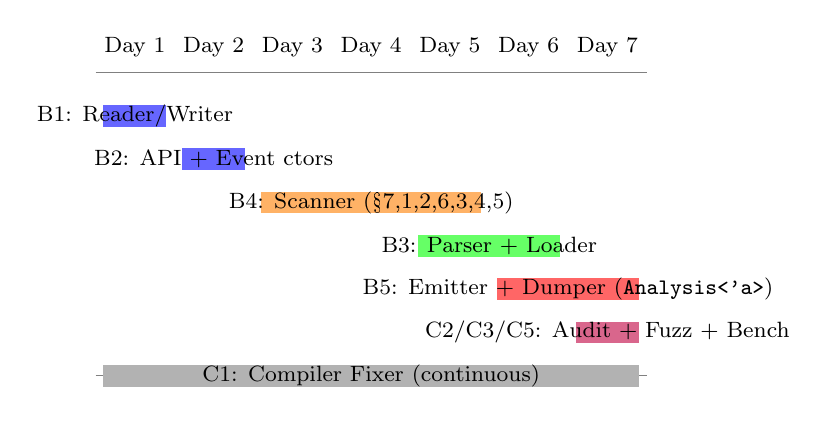
\begin{tikzpicture}[
  x=1.0cm, y=0.55cm,
  every node/.style={font=\footnotesize}
]
\foreach \d in {1,2,3,4,5,6,7} \node at (\d, 0.6) {Day \d};
\draw[thin, gray] (0.5,0) -- (7.5,0);
\draw[thin, gray] (0.5,-7) -- (7.5,-7);
\def\bar#1#2#3#4#5{%
  \fill[#5!60] (#1-0.4,-#3+0.25) rectangle (#2+0.4,-#3-0.25);
  \node at ({(#1+#2)/2}, -#3) {#4};
}
\bar{1}{1}{1}{B1: Reader/Writer}{blue}
\bar{2}{2}{2}{B2: API + Event ctors}{blue}
\bar{3}{5}{3}{B4: Scanner (\S 7,1,2,6,3,4,5)}{orange}
\bar{5}{6}{4}{B3: Parser + Loader}{green}
\bar{6}{7}{5}{B5: Emitter + Dumper (\texttt{Analysis<'a>})}{red}
\bar{7}{7}{6}{C2/C3/C5: Audit + Fuzz + Bench}{purple}
\bar{1}{7}{7}{C1: Compiler Fixer (continuous)}{gray}
\end{tikzpicture}
\end{center}

% =====================================================================
\phantomsection
\addcontentsline{toc}{section}{Appendix B. Environmental prerequisites}
\refstepcounter{section}\label{app:env}
\section*{Appendix B. Environmental prerequisites}

\begin{itemize}
\item Rust 1.86 stable + nightly (for Miri, cargo-careful).
\item Clang $\ge 18$ + LLVM $\ge 18$ (c2rust target).
\item CMake $\ge 3.20$ (for libyaml C build).
\item c2rust $\ge 0.21$.
\item AFL++ $\ge 4.20$.
\item cargo-fuzz, cargo-careful, kani-verifier, cbindgen
(installable via \texttt{cargo install}).
\item Python $\ge 3.10$ (for the ABI-diff normalizer; see
\Cref{app:abidiff}).
\item A copy of the \texttt{yaml/yaml-test-suite} repository.
\item A copy of the \texttt{yaml/libyaml} repository, built as a shared
object.
\item For libexpat phase: \texttt{libexpat/libexpat} repository,
W3C \texttt{xmlconf} test suite.
\end{itemize}

% =====================================================================
\phantomsection
\addcontentsline{toc}{section}{Appendix C. The ABI-diff normalizer}
\refstepcounter{section}\label{app:abidiff}
\section*{Appendix C. The ABI-diff normalizer}

The script \texttt{scripts/abi\_diff.py} referenced in
Appendix~A.4 is reproduced verbatim below. Its job is to read a
clang-format-normalized, comment-stripped C header from standard
input, parse it into top-level declarations (\texttt{typedef},
\texttt{struct}, \texttt{enum}, function prototype), sort the
declarations alphabetically by their leading identifier, and emit
the sorted result on standard output. The script is intentionally
tiny so that the entire ABI-parity check is auditable.

\begin{lstlisting}[language=,basicstyle=\ttfamily\footnotesize]
#!/usr/bin/env python3
"""abi_diff.py --sort
Read a (clang-format'ed, comment-stripped) C header from stdin,
sort its top-level declarations by leading identifier, write to
stdout. Used by the ABI-parity check in Appendix A.4.
"""
import re
import sys

SRC = sys.stdin.read()

# Split on a blank line OR on a top-level closing semicolon
# followed by newline. Keep the delimiter at the end of each chunk.
chunks = re.split(r'(?<=;)\n(?=\S)|\n\n+', SRC.strip())

def key(chunk: str) -> str:
    # Find the longest contiguous identifier in the chunk; that is
    # almost always the typedef/struct/function name we care about.
    idents = re.findall(r'[A-Za-z_][A-Za-z0-9_]*', chunk)
    # Skip C keywords that are not declaration names.
    skip = {'typedef','struct','union','enum','const','static',
            'extern','void','int','char','unsigned','signed',
            'short','long','float','double','size_t'}
    for tok in idents:
        if tok not in skip:
            return tok
    return idents[0] if idents else ''

if '--sort' in sys.argv[1:]:
    chunks.sort(key=key)

print('\n\n'.join(c.strip() for c in chunks if c.strip()))
\end{lstlisting}

\end{document}
